\documentclass[preprint,1p,authoryear]{elsarticle}

% ===== Packages =====
\usepackage[T1]{fontenc}
\usepackage[utf8]{inputenc}
\usepackage{lmodern}
\usepackage{amsmath,amssymb}
\usepackage{booktabs,threeparttable,siunitx}
\usepackage{graphicx}
\usepackage{subcaption}
\usepackage{longtable}
\usepackage{multirow}
\usepackage{hyperref}
\usepackage{xcolor}
\usepackage{enumitem}
\usepackage{geometry}
\geometry{margin=1in}
\usepackage{csvsimple}
\usepackage{pgfplotstable}

% Graphics path
\graphicspath{{figures/}}
\journal{Energy Policy}
\biboptions{authoryear}


% ===== Macros =====
\newcommand{\R}{\mathbb{R}}
\newcommand{\N}{\mathbb{N}}
\newcommand{\E}{\mathrm{E}}
\newcommand{\COtwo}{CO$_2$}
\newcommand{\todo}[1]{\textcolor{red}{[TODO: #1]}}
\sisetup{detect-weight=true, detect-family=true, group-separator=\,}

% ===== Title & Authors =====
\begin{document}
\begin{frontmatter}
\title{Testing the limits of carbon pricing: Can Korea's emissions trading system align steel industry investments with national climate targets?}

\author[planit]{Jinsu Park}
\address[planit]{PLANiT Institute, Seoul, Republic of Korea}

% ===== Highlights (Energy Policy requires 3--5 bullet highlights) 

\section*{Highlights}
\begin{itemize}[leftmargin=*]
  \item \textbf{Integrated policy assessment}: We couple a mixed-integer optimisation model with NGFS carbon-price pathways to test K-ETS adequacy against POSCO's 1,110~MtCO$_2$ sectoral budget (2025--2050).
  \item \textbf{Updated NGFS pricing}: Net Zero 2050 reaches \$150/tCO$_2$ by 2030 and \$450/tCO$_2$ by 2050; Below~2$^\circ$C attains \$80/tCO$_2$ and \$240/tCO$_2$; the NDC case plateaus at \$40/tCO$_2$ and \$100/tCO$_2$.
  \item \textbf{Persistent budget overshoot}: Even under Net Zero 2050, cumulative emissions reach 1,190~MtCO$_2$ (+7\%), revealing that current trajectories remain insufficient without complementary reforms.
  \item \textbf{CCUS plus scrap required}: Only once the ETS price exceeds \$110/tCO$_2$ do scrap-EAF shares climb, and prices above \$165/tCO$_2$ unlock CCUS retrofits that supply 51\% of 2050 output—highlighting infrastructure gaps on both routes.
  \item \textbf{No-CCUS sensitivity}: Disabling capture under Net Zero pushes cumulative emissions to 1,324~MtCO$_2$ (+19\%) and shifts 36\% of output to hydrogen DRI while quadrupling ETS liabilities.
  \item \textbf{Policy focus}: Budget alignment demands price floors rising toward \$500/tCO$_2$, accelerated free-allocation phase-out, targeted support for scrap logistics plus CO$_2$ infrastructure, and CCfDs that de-risk low-carbon steel investment.
\end{itemize}

% ===== Abstract =====
\begin{abstract}
Can carbon pricing alone deliver the deep industrial decarbonisation required for climate neutrality? We investigate this question for Korea's steel sector—responsible for roughly 10\% of national emissions—using a mixed-integer optimisation model of POSCO's technology portfolio. We update the analysis with internally consistent NGFS carbon-price pathways (Net Zero 2050: \$150/tCO$_2$ in 2030 and \$450/tCO$_2$ in 2050; Below~2$^\circ$C: \$80/tCO$_2$ and \$240/tCO$_2$; NDCs: \$40/tCO$_2$ and \$100/tCO$_2$) and reassess investment behaviour against a 1,110~MtCO$_2$ budget (2025--2050). Current trajectories remain inadequate: cumulative emissions reach 1,190~MtCO$_2$ (+7\%) under Net Zero 2050, 1,713~MtCO$_2$ (+54\%) under Below~2$^\circ$C, and 1,981~MtCO$_2$ (+78\%) under the NDC case. The cost-minimising Net Zero portfolio couples extensive CCUS retrofits (51\% of 2050 output) with scrap-based electric arc furnaces capped at 36\%, while hydrogen routes stay uneconomic at baseline costs. A no-CCUS sensitivity along the Net Zero price path pushes cumulative emissions to 1,324~MtCO$_2$ (+19\%), with hydrogen DRI rising to 36\% of output but ETS liabilities quadrupling to \$43~billion. Achieving budget compliance therefore requires higher and more credible price floors, faster free-allocation phase-out, and complementary infrastructure policies that unlock scrap supply chains as well as CO$_2$ transport and storage.
\end{abstract}

\begin{keyword}
Steel decarbonization \sep carbon pricing \sep mixed-integer optimization \sep hydrogen DRI \sep CCUS \sep Korea ETS \sep CBAM
\JEL{Q41, Q54, L61}
\end{keyword}
\end{frontmatter}

% ===== 1. Introduction =====
\section{Introduction}

Can market-based climate policies deliver the massive industrial transformation required for net-zero emissions? This question has become increasingly urgent as governments worldwide deploy carbon pricing to decarbonize energy-intensive industries. Despite the proliferation of emissions trading systems covering millions of firms across dozens of countries, we still lack robust empirical evidence on whether carbon prices can actually drive the deep technological shifts required to meet climate targets \citep{Green2021}. This paper addresses that gap by testing whether Korea's carbon pricing system can align steel industry investments with national climate commitments.

The stakes are particularly high in steel production, which accounts for roughly 7\% of global CO$_2$ emissions \citep{worldsteel2022}. Korea's steel sector offers an especially revealing test case. As the world's sixth-largest producer, Korea's industry is dominated by a single firm—POSCO—whose emissions alone represent 10\% of the nation's greenhouse gas inventory \citep{KOSIS2023}. To put this in perspective, POSCO's annual emissions exceed those of entire countries like Belgium or Chile. This industrial concentration creates both an opportunity and a challenge: if carbon pricing cannot drive transformation in such a focused, high-emission sector with clear policy leverage, its prospects for broader industrial decarbonization look questionable.

What makes steel particularly challenging is the sheer scale of technological disruption required. Moving from today's carbon-intensive blast furnace routes to low-carbon alternatives—whether hydrogen-based direct reduction, carbon capture and storage, or electric arc furnaces powered by clean electricity—demands wholesale replacement of production infrastructure \citep{IEA2020steel}. Individual plant investments often exceed \$2 billion, and once built, these facilities operate for 25 to 40 years \citep{MaterialEconomics2019}. The lumpy and irreversible nature of these capital decisions creates powerful inertia that carbon price signals must overcome. A steel company cannot gradually shift its production mix the way a power generator can dispatch different plants; it must commit to discrete, long-lived technology choices that lock in emission trajectories for decades.

Korea's policy landscape provides a compelling context for examining these dynamics. The Korean Emissions Trading System (K-ETS), launched in 2015, now covers 70\% of national emissions including the steel sector \citep{kim2021kets}. However, the system has historically operated with generous free allocation—POSCO received allowances covering approximately 95\% of its emissions in recent years \citep{ICAP2024}—effectively insulating the sector from carbon costs. This protection is scheduled to decline as Korea pursues its 2030 nationally determined contribution (a 40\% reduction from 2018 levels) and 2050 carbon neutrality goal, gradually exposing steel producers to meaningful carbon price signals. The question is whether this evolving price trajectory will prove sufficient to drive the necessary investment response.

To frame this question more precisely, we need to establish what "sufficient" means in climate terms. Korea's carbon neutrality framework implies a finite carbon budget for each economic sector \citep{korea2020carbon}. Drawing on Korea's national climate commitments and standard burden-sharing principles, we estimate that the steel sector can emit approximately 1,850 MtCO$_2$ between 2025 and 2050 while remaining consistent with national targets. Given POSCO's roughly 60\% share of domestic steel production, this translates to a firm-level budget of about 1,110 MtCO$_2$ over the period. The fundamental test of carbon pricing adequacy, then, is whether profit-maximizing corporate investment decisions—responding to planned carbon price trajectories—will stay within this budget envelope. Section 3 provides full details on our budget derivation methodology.

We examine this question using a mixed-integer linear programming model that optimizes POSCO's technology portfolio under three carbon price scenarios drawn from the Network for Greening the Financial System (NGFS) \citep{NGFS2024}. These globally consistent scenarios—Net Zero 2050, Below 2$^\circ$C, and NDCs—reflect different levels of climate ambition and are widely used by central banks and financial regulators for climate risk assessment. Our model minimizes the net present value of total system costs (capital expenditure, operating costs, and carbon compliance costs) subject to realistic constraints on technology deployment, feedstock availability, and product quality. Unlike previous steel optimization studies that treat capacity additions as continuous variables, we explicitly model the discrete, lumpy nature of blast furnace investment cycles. By comparing the resulting emission pathways against our derived carbon budget, we can assess whether current carbon pricing trajectories actually align industrial investment incentives with climate targets.

Our central hypothesis is that carbon pricing alone, even at ambitious levels, will prove insufficient to achieve sectoral carbon budget compliance. Specifically, we expect that the Net Zero 2050 price trajectory—reaching \$150/tCO$_2$ by 2030 and \$450/tCO$_2$ by 2050—represents a necessary but still inadequate condition for staying within budget, due to capital stock inertia, infrastructure constraints, and technology cost barriers. Meanwhile, carbon pricing consistent with current policy trajectories (the NDCs scenario, reaching only \$40/tCO$_2$ by 2030 and \$100/tCO$_2$ by 2050) should systematically overshoot budget allocations, creating a dangerous policy-performance gap that undermines national climate commitments. If confirmed, this hypothesis would point to fundamental limitations in relying on carbon pricing as the primary instrument for industrial decarbonization.

Our results provide sobering confirmation of these concerns. Even under the most aggressive carbon price scenario—Net Zero 2050—POSCO's cumulative emissions still overshoot the carbon budget by 80 MtCO$_2$, or roughly 7\%. The Below 2$^\circ$C pathway produces a 603 MtCO$_2$ overshoot (+54\%), while the NDC scenario leads to an 871 MtCO$_2$ excess (+78\%). These overshoots occur despite the model's assumption of perfect foresight, rational optimization, and full technology availability—conditions far more favorable than real-world circumstances. The findings suggest that current carbon pricing trajectories are fundamentally inadequate for achieving climate targets in energy-intensive industries. Meeting those targets will require not just higher carbon prices, but also complementary policies that address infrastructure gaps, accelerate free allocation phase-outs, and reduce investment risks for low-carbon technologies. The remainder of this paper develops these arguments in detail and explores their implications for climate policy design.

\section{Literature Review}

Understanding whether carbon pricing can drive industrial decarbonization requires synthesizing insights from three distinct research traditions that have largely developed in isolation. Engineering studies have mapped out technically feasible decarbonization pathways for steel production, identifying promising technologies but often treating policy instruments as exogenous parameters. Economic analyses have examined carbon pricing effectiveness in regulated industries, yet systematic evidence on heavy manufacturing remains surprisingly thin. Meanwhile, climate scientists have developed increasingly sophisticated carbon budget frameworks, but translating these global constraints into operational sectoral targets has proven elusive. The central gap—and the one this paper addresses—is that no existing research rigorously tests whether carbon pricing trajectories aligned with climate targets can actually drive the technology transitions required to meet sectoral carbon budgets. We begin by reviewing each literature stream in turn, highlighting both their contributions and limitations, before positioning our approach at their intersection.

\subsection{Steel sector decarbonization: Technology pathways and constraints}

Research on steel decarbonization has matured considerably over the past decade, evolving from single-technology assessments to system-level analyses that grapple with real-world constraints. The foundational work established a taxonomy of three main decarbonization routes \citep{IEA2020steel}: carbon management through retrofitting carbon capture and storage (CCUS) to existing blast furnace-basic oxygen furnace (BF-BOF) facilities; circularity and electrification via expanded use of scrap-based electric arc furnaces (EAF); and hydrogen-based direct reduction that replaces coking coal with H$_2$ as the primary reductant. This classification remains useful, though increasingly we recognize that real decarbonization strategies will likely combine elements from all three routes rather than betting on a single pathway.

Early techno-economic studies focused primarily on demonstrating technical feasibility and comparing levelized costs across technologies under static assumptions \citep{Vogl2018, Otto2017}. These analyses were valuable in establishing baseline cost estimates, but they treated technology costs as fixed and assumed perfect availability of necessary inputs—both problematic assumptions for long-term scenario analysis. More recent work has begun incorporating dynamic factors that matter critically for deployment. For instance, \citet{prammer2021steel} examined how technology learning curves might reduce hydrogen DRI costs over time, while \citet{ueckerdt2021potential} explored the co-evolution of hydrogen infrastructure and end-use applications. System-level constraints have also received growing attention: \citet{pauliuk2013global} documented global scrap availability limits that constrain how much steel production can shift to EAF routes, and \citet{wang2021hydrogen} mapped renewable hydrogen production potential, finding substantial regional variation in availability and cost. The most comprehensive synthesis came from \citet{MaterialEconomics2019}, whose European steel roadmap emphasized that decarbonization pathways depend critically on the timing and sequencing of policy interventions—get the timing wrong, and you risk either stranded assets or locked-in emissions.

Despite this progress, three important limitations remain. First, nearly all existing optimization models treat technology adoption as continuous decision variables that can be adjusted incrementally. This overlooks the fundamentally lumpy and irreversible nature of steel industry investment \citep{Griffin2020}. Blast furnaces are built as discrete units with 40-year lifespans; companies cannot simply adopt "30\% of a hydrogen DRI plant." This matters because it introduces path dependencies and option values that continuous models miss entirely. Second, while some studies examine specific regions, few integrate the full set of region-specific factors—policy frameworks, feedstock availability, infrastructure constraints, and industrial structure—that jointly shape feasible decarbonization pathways \citep{zhang2022steel}. A technology sequence that works for European steel may not transfer to Korea's context. Third, and most critically for our purposes, existing studies evaluate decarbonization scenarios against arbitrary emission targets or cost minimization objectives, but not against carbon budgets derived systematically from national climate commitments. Yet assessing whether policy instruments can deliver on actual climate targets is precisely what policymakers need to know.

\subsection{Carbon pricing effectiveness in energy-intensive industries}

If the steel engineering literature has made substantial progress, the same cannot be said for empirical evidence on carbon pricing effectiveness in heavy industry. The broader carbon pricing literature has documented responsiveness in sectors with relatively flexible production: power generation shows clear price sensitivity \citep{jarke2017carbon}, and oil refineries have adjusted product slates in response to EU ETS prices \citep{fowlie2016carbon}. But these sectors differ fundamentally from energy-intensive manufacturing, where production technologies are capital-intensive, long-lived, and offer limited short-run substitution possibilities.

For manufacturing specifically, the evidence remains limited and somewhat contradictory. \citet{calel2016innovation} found that EU ETS coverage accelerated low-carbon patenting in participating firms, suggesting that carbon pricing can stimulate innovation even if near-term abatement options are limited. However, \citet{martin2016industry} documented substantial emissions leakage, with regulated firms shifting production to unregulated facilities rather than reducing emissions intensity. This divergence hints at an important distinction: carbon pricing may change innovation incentives without necessarily changing near-term production and investment decisions, especially when free allocation shields firms from carbon costs.

The steel sector presents an even more challenging test case. \citet{sartor2012benchmark} showed that Phase III EU ETS free allocation—based on product-specific benchmarks—effectively removed carbon cost exposure for most steel producers, leaving them with little incentive to invest in new technologies despite rising carbon prices. Even when firms face carbon costs, price levels matter enormously. \citet{demailly2018european} estimated that carbon prices would need to exceed €50 per tonne CO$_2$ to make hydrogen-based DRI competitive with conventional blast furnaces at prevailing technology costs—a threshold the EU ETS only briefly reached during the 2008 financial crisis before collapsing. Whether the price levels now being contemplated for 2030 and beyond will prove sufficient remains an open question.

Research on emerging market carbon pricing systems has begun to fill in the picture, though the findings so far are not encouraging. \citet{kim2021kets} documented the first five years of Korea's emissions trading system, finding limited price discovery, persistent price suppression due to regulatory intervention, and minimal evidence of industrial restructuring. \citet{wang2021carbon} reported similar patterns in China's ETS pilots: prices remained low, volatility was high, and covered firms showed little change in investment behavior. These studies raise a troubling possibility: carbon pricing may be a necessary component of industrial climate policy, but current implementations often fail to generate the price signals needed to drive transformation.

What remains missing from this literature is any rigorous empirical test of whether planned carbon price trajectories—the ones actually embedded in national climate policies—can drive technology adoption at the scale and pace required for sectoral carbon budget compliance. Existing studies either examine historical behavior under low and uncertain carbon prices, or perform stylized analyses using arbitrary price assumptions disconnected from actual policy commitments. Neither approach answers the policy-relevant question: are current plans adequate?

\subsection{Sectoral carbon budgets and allocation mechanisms}

The concept of carbon budgets has become central to climate policy, yet its application to sectoral planning remains underdeveloped. The intellectual foundation came from climate science, particularly the finding that cumulative carbon emissions determine long-run temperature outcomes with remarkable precision \citep{matthews2009proportionality}. This relationship implies that limiting warming to any target requires staying within a finite "budget" of allowable emissions—a constraint that fundamentally changes how we think about climate policy.

Translating global budgets into actionable policy has proven challenging at multiple levels. At the global scale, \citet{rogelj2019new} refined estimates of remaining carbon budgets consistent with 1.5°C and 2°C temperature limits, accounting for recent emissions and updated climate sensitivities. But as \citet{millar2017emission} emphasized, meeting these budgets depends critically on near-term emission trajectories; delayed action rapidly erodes the remaining budget available for later decades. Moving from global to national budgets introduces thorny equity questions about how to allocate a finite resource across countries with vastly different historical responsibilities and development needs \citep{raupach2014sharing}. \citet{robiou2019national} proposed various allocation principles—equal per capita, grandfathering, capacity-based—each with different ethical foundations and practical implications.

Sectoral carbon budget allocation adds yet another layer of complexity \citep{gasser2018negative}. Should sectors with limited abatement options receive larger allocations? How should we account for differences in decarbonization costs, trade exposure, and social importance? \citet{kuramochi2018beyond} examined sectoral decomposition approaches, but struggled to identify clear principles for allocation that are both technically sound and politically acceptable. The practical result is that most national climate strategies remain vague about sectoral targets, offering aspirational goals rather than binding budgets.

For steel specifically, the stakes are particularly high. Given the sector's emissions intensity and the long lifetimes of production assets, \citet{bataille2018role} estimated that steel production could consume 15-20\% of the remaining global carbon budget under business-as-usual trajectories—far exceeding the sector's share of current GDP or employment. This raises urgent questions about how aggressive steel decarbonization must be, and whether available policy instruments can deliver the necessary transformation. \citet{Griffin2020} emphasized that sectoral carbon budgets should guide industrial policy design, yet acknowledged that we lack clear frameworks for deriving these budgets or assessing policy adequacy against them.

The fundamental gap is empirical: no existing research has tested whether current policy instruments—carbon pricing in particular—can actually deliver outcomes consistent with sectorally allocated carbon budgets. Without such tests, we cannot know whether planned policies are on track or require fundamental recalibration. This gap is especially concerning for energy-intensive industries like steel, where transformation timelines are long and getting policies wrong carries enormous consequences.

\subsection{Research contribution and positioning}

This study addresses the gaps identified above by integrating engineering-economic optimization with top-down carbon budget constraints to test carbon pricing adequacy in heavy industry. We make three main contributions.

First, we develop an integrated methodological framework that combines bottom-up technology optimization with carbon budget evaluation. Unlike previous steel optimization models that treat investments as continuous or use arbitrary emission targets, our mixed-integer formulation captures the discrete, lumpy nature of blast furnace campaigns while benchmarking results against carbon budgets derived systematically from national climate commitments. This allows us to quantify "policy-performance gaps"—the difference between what current policies are likely to deliver and what climate targets require.

Second, we provide what is, to our knowledge, the first quantitative assessment of whether carbon price trajectories aligned with major climate scenarios can drive technology transitions consistent with sectoral carbon budgets. Using Korea's steel sector as an empirically rich case study, we test three carbon price pathways from the Network for Greening the Financial System: Net Zero 2050, Below 2°C, and NDCs. This design directly addresses the question policymakers face: are our current plans sufficient, or do we need more aggressive policy intervention?

Third, we generate actionable policy insights by identifying specific carbon price thresholds that trigger different technology transitions and quantifying the magnitude of reforms needed to close emerging policy-performance gaps. Beyond simply documenting inadequacy, we provide guidance on what would be required for budget compliance—higher price floors, faster free allocation phase-outs, and complementary infrastructure policies.

Our approach bridges engineering-economic modeling with climate policy evaluation in a way that can extend to other energy-intensive sectors and jurisdictions. However, we should be clear about limitations. We focus on a single firm in one country, which limits generalizability though offers the advantage of institutional and technological specificity. We assume perfect foresight and cost-minimizing behavior, whereas real investment decisions involve uncertainty, organizational inertia, and multiple objectives beyond cost minimization. We do not model political economy constraints on carbon pricing—such as lobbying, public acceptance, or international competitiveness concerns—that often bind more tightly than technical or economic constraints. Finally, our discrete-time formulation (annual periods) cannot capture intra-year dynamics or the precise timing of investment campaigns. Despite these limitations, we believe the framework provides valuable insights into carbon pricing adequacy and establishes a template for policy evaluation that future research can refine and extend.

% ===== 2. Methods: Optimization model =====
\section{Methodology}

Our analytical approach combines engineering-economic optimization with climate policy evaluation to test a straightforward but consequential question: can carbon pricing alone drive industrial transformation at the pace required to meet climate targets? We answer this by building a detailed model of POSCO's technology investment decisions under different carbon price scenarios, then comparing the resulting emission pathways against sectoral carbon budgets derived from Korea's climate commitments. This section first outlines our conceptual framework, then develops the optimization model in detail, and finally describes how we assess policy-performance gaps.

\subsection{Conceptual framework and model overview}

Our analysis proceeds across three integrated levels, each addressing a distinct analytical question:

\textbf{Level 1: Technology Portfolio Optimization.} What technology mix would a cost-minimizing steel producer choose under different carbon price scenarios? We use a mixed-integer linear programming (MILP) model to determine POSCO's least-cost technology adoption pathway from 2025 to 2050. The model explicitly captures three features critical for industrial decarbonization: lumpy investment decisions (you cannot build half a blast furnace), long-lived assets (plants operate for 25-40 years), and operational constraints (capacity utilization limits, feedstock availability, product quality requirements). By solving this optimization problem under alternative carbon price trajectories, we can trace out how investment behavior responds to policy signals.

\textbf{Level 2: Carbon Budget Derivation.} What emission pathway is consistent with Korea's climate commitments? We derive a sectoral carbon budget for steel production using proportional allocation based on the sector's current emissions share and Korea's nationally determined contribution (NDC) reduction targets for 2030 and 2050 carbon neutrality goals. This budget represents the cumulative emissions envelope that the steel sector can occupy while remaining consistent with national climate targets. By allocating this sectoral budget proportionally to POSCO based on market share, we establish a firm-level carbon constraint against which to evaluate technology pathways.

\textbf{Level 3: Policy-Performance Gap Assessment.} Does profit-maximizing investment behavior stay within climate-consistent carbon budgets? We compare the optimized emission pathways from Level 1 against the carbon budget constraints from Level 2. The difference—what we term the "policy-performance gap"—quantifies whether carbon pricing trajectories are adequate for climate target compliance. Positive gaps indicate systematic overshooting where current policies fall short; zero or negative gaps would indicate budget compliance.

This multi-level framework enables rigorous testing of our central hypothesis: that current carbon pricing trajectories, even ambitious ones, prove inadequate for sectoral carbon budget compliance without complementary policies. The beauty of this approach is its transparency—by separating technology optimization from budget evaluation, we can clearly identify where policy-performance gaps emerge and what would be required to close them.

\subsection{Optimization model formulation}

The core of our analysis is an optimization model that determines POSCO's least-cost technology portfolio over a 25-year planning horizon. Think of this as solving the company's long-term investment problem: given projected demand for steel, commodity prices, technology costs, and carbon prices, which production technologies should the firm invest in and when? The model minimizes total system costs—capital expenditure for new facilities, operating costs for production, and carbon compliance costs—subject to realistic constraints on technology deployment, feedstock availability, and operational limits.

What makes this model distinctive is its treatment of investment discreteness. Unlike many energy system models that allow fractional capacity additions, we recognize that steel plants come in discrete lumps—blast furnaces are built as complete units with typical capacities of 4 million tonnes per year, not as smoothly adjustable variables. This matters because it introduces path dependencies: once you build a blast furnace, you are locked into its technology and emission profile for decades. The model captures this reality through integer decision variables that force the optimizer to make discrete yes/no choices about building new capacity.

We now develop the mathematical formulation systematically, starting with notation and building toward the complete optimization problem.

\subsubsection{Sets and indices}

The model operates over discrete time periods and technology alternatives:

\begin{itemize}[leftmargin=*]
    \item $t \in \mathcal{T}$: years, $t = 2025, \dots, 2050$. We use annual time steps to balance computational tractability with sufficient granularity to capture investment timing.
    \item $r \in \mathcal{R}$: production routes, including BF--BOF (conventional blast furnace), BF--BOF+CCUS (with carbon capture), Scrap-EAF (electric arc furnace using scrap), NG-DRI--EAF (natural gas direct reduction), and H$_2$-DRI--EAF (hydrogen direct reduction). These five routes span the full spectrum of steel decarbonization options from incumbent technologies to emerging alternatives.
    \item $\mathcal{R}^{CCUS} \subseteq \mathcal{R}$: subset of routes equipped with CCUS technology, enabling the model to distinguish carbon management options.
    \item $\mathcal{R}^{H_2} \subseteq \mathcal{R}$: subset of hydrogen-based routes, allowing us to impose technology readiness constraints on emerging pathways.
\end{itemize}

\subsubsection{Decision variables}

The model determines four types of decisions:

\begin{itemize}[leftmargin=*]
    \item $B_{r,t} \in \mathbb{Z}_{\ge 0}$: number of units of production route $r$ built in year $t$. The integer constraint reflects investment lumpiness—you build whole plants, not fractions of plants.
    \item $K_{r,t} \in \mathbb{R}_{\ge 0}$: available production capacity of route $r$ in year $t$ (Mt/y). This evolves based on investment decisions and reflects the cumulative build-out of each technology.
    \item $Q_{r,t} \in \mathbb{R}_{\ge 0}$: annual production from route $r$ in year $t$ (Mt). The model can operate facilities below full capacity to minimize costs, subject to utilization constraints.
    \item $ETS_{t}^{+} \in \mathbb{R}_{\ge 0}$: net emissions trading system liability in year $t$ (Mt CO$_2$), representing the carbon allowances the firm must purchase after accounting for free allocation.
\end{itemize}

Together, these variables let the model choose not just what technologies to deploy, but when to deploy them and how intensively to operate them—all in response to evolving carbon prices and input costs.

\subsubsection{Objective function}

The optimization minimizes the net present value of total system costs over the planning horizon:

\begin{align}
\min_{B,K,Q,ETS^+} \; & \sum_{t \in \mathcal{T}} \delta_t \left[ C^{CAPEX}_t + C^{FixedOM}_t + C^{VarOPEX}_t + C^{ETS}_t \right],
\end{align}

where $\delta_t = (1+\rho)^{-(t-t_0)}$ is the discount factor with real discount rate $\rho = 0.05$ and base year $t_0 = 2025$. The 5\% discount rate reflects typical corporate hurdle rates for long-term industrial investments and is consistent with IEA energy system modeling practice.

Each cost component captures a distinct economic consideration:

\textit{Capital expenditure} reflects upfront investment costs for new production capacity:
\begin{align}
C^{CAPEX}_t &= \sum_{r \in \mathcal{R}} B_{r,t} \cdot \kappa_r \cdot c^{capex}_r \cdot 10^6, \label{eq:capex}
\end{align}
where $\kappa_r$ denotes unit capacity (Mt/y) for route $r$, and $c^{capex}_r$ represents technology-specific capital costs (USD/tpy). The discrete nature of $B_{r,t}$ means CAPEX comes in lumps rather than smoothly—a key feature distinguishing our model from continuous approaches.

\textit{Fixed operating costs} cover capacity-related expenses independent of utilization:
\begin{align}
C^{FixedOM}_t &= \sum_{r \in \mathcal{R}} K_{r,t} \cdot c^{fixom}_r \cdot 10^6, \label{eq:fixom}
\end{align}
where $c^{fixom}_r$ denotes fixed O\&M costs (USD/tpy/y). These capture maintenance, labor, and overhead expenses that must be paid regardless of production levels.

\textit{Variable operating costs} reflect input commodity expenses that scale with production:
\begin{align}
C^{VarOPEX}_t &= \sum_{r \in \mathcal{R}} Q_{r,t} \cdot \left( \sum_{i \in \mathcal{I}} \alpha_{r,i} \cdot p_{i,t} \right) \cdot 10^6, \label{eq:varopex}
\end{align}
where $\alpha_{r,i}$ represents input intensity of commodity $i$ for route $r$ (physical units per tonne steel), and $p_{i,t}$ denotes commodity prices (USD per physical unit). The commodity set includes $\mathcal{I} = \{$iron ore, coking coal, scrap steel, natural gas, electricity, hydrogen, fluxes, alloys$\}$. This detailed representation allows the model to capture feedstock substitution across routes—for instance, hydrogen replacing coking coal in DRI processes.

\textit{Carbon compliance costs} reflect emissions trading system obligations:
\begin{align}
C^{ETS}_t &= P^{CO_2}_t \cdot ETS_t^+ \cdot 10^6, \label{eq:ets}
\end{align}
where $P^{CO_2}_t$ is the carbon price (USD/tCO$_2$) following NGFS scenario trajectories. This cost only applies to net emissions after free allocation, capturing the partial cost exposure under current K-ETS design.

The objective function thus balances multiple economic considerations: avoiding large upfront capital costs, minimizing ongoing operating expenses, and managing carbon compliance liabilities. The model's cost-minimizing logic reflects how rational firms would respond to price signals, making it a useful tool for assessing policy effectiveness.

\subsubsection{Constraints: Ensuring realistic technology transitions}

The optimization is subject to multiple constraint sets that ensure the solution reflects engineering realities and policy boundaries. We organize these into three categories: material balance and production constraints, emissions and carbon pricing rules, and technology deployment constraints.

\textbf{Material balance and production constraints} ensure the model produces enough steel while respecting capacity limits:

\textit{Demand satisfaction:} Total production must meet exogenous steel demand in each period:
\begin{align}
\sum_{r \in \mathcal{R}} Q_{r,t} &= D_t, \quad \forall t \in \mathcal{T}, \label{eq:demand}
\end{align}
where $D_t$ denotes steel demand (Mt/y) following the trajectory described in Section~4.4. This constraint abstracts from competitive dynamics to focus on technology transition incentives, assuming POSCO maintains market share.

\textit{Capacity utilization:} Production from each route cannot exceed available capacity times a maximum utilization factor:
\begin{align}
Q_{r,t} &\le \mu \cdot K_{r,t}, \quad \forall r \in \mathcal{R}, t \in \mathcal{T}, \label{eq:utilization}
\end{align}
where $\mu = 0.90$ represents realistic capacity utilization accounting for maintenance schedules, operational flexibility, and quality considerations. This prevents the model from assuming 100\% utilization, which would be operationally infeasible.

\textit{Capacity evolution:} Available capacity evolves based on investment decisions and retirements:
\begin{align}
K_{r,t} &= K_{r,t-1} + \kappa_r \cdot B_{r,t} - R_{r,t}, \quad \forall r \in \mathcal{R}, t \in \mathcal{T} \setminus \{t_0\}, \label{eq:capacity}
\end{align}
where $R_{r,t}$ represents capacity retirements based on assumed 40-year asset lifetimes for blast furnaces and 30-year lifetimes for other routes. Initial conditions are set to match POSCO's current capacity configuration:
\begin{align}
K_{r,t_0} &= K_r^{initial}, \quad \forall r \in \mathcal{R}. \label{eq:initial}
\end{align}

\textbf{Emissions and carbon pricing constraints} translate production decisions into carbon costs:

\textit{ETS liability:} The model calculates net carbon liabilities after accounting for free allocation:
\begin{align}
ETS_t^+ &\ge \sum_{r \in \mathcal{R}} ef_r^{net} \cdot Q_{r,t} - A_t^{free}, \quad \forall t \in \mathcal{T}, \label{eq:ets_balance}
\end{align}
where $ef_r^{net}$ denotes net emission factors (tCO$_2$/t steel) and $A_t^{free}$ specifies free allocation under K-ETS declining schedules. The inequality formulation allows $ETS_t^+ = 0$ when free allocation exceeds emissions, but prevents negative values (no allowance banking).

\textit{CCUS emission reduction:} For routes equipped with carbon capture, net emissions are reduced by the capture efficiency:
\begin{align}
ef_r^{net} &= ef_r^{gross} \cdot (1 - \eta^{CCUS}), \quad \forall r \in \mathcal{R}^{CCUS}, \label{eq:ccus_factor}
\end{align}
where $\eta^{CCUS} = 0.80$ represents capture efficiency based on current post-combustion technology performance. For routes without CCUS, net emissions equal gross emissions:
\begin{align}
ef_r^{net} &= ef_r^{gross}, \quad \forall r \in \mathcal{R} \setminus \mathcal{R}^{CCUS}. \label{eq:no_ccus}
\end{align}

\textbf{Technology deployment constraints} enforce realistic timing and discrete investment:

\textit{Technology readiness:} Emerging technologies cannot be deployed before reaching commercial readiness:
\begin{align}
B_{r,t} &= 0, \quad \forall r \in \mathcal{R}^{H_2}, t < 2030, \label{eq:h2_timing}\\
\sum_{r \in \mathcal{R}^{CCUS}} B_{r,t} &= 0, \quad \forall t < 2027, \label{eq:ccus_timing}
\end{align}
reflecting POSCO's stated demonstration timelines: CCUS pilot completion by 2027 and hydrogen DRI commercial deployment from 2030. These constraints prevent the model from prematurely adopting unproven technologies.

\textit{Investment discreteness:} Capacity additions must be integer multiples of standardized plant sizes:
\begin{align}
B_{r,t} &\in \mathbb{Z}_{\ge 0}, \quad \forall r \in \mathcal{R}, t \in \mathcal{T}. \label{eq:integer}
\end{align}
This constraint captures the lumpy nature of steel industry investment and creates path dependencies absent in continuous models.

Together, these constraints ensure the optimization produces realistic technology transitions that respect engineering limits, policy parameters, and commercial readiness—not just theoretically optimal but practically infeasible solutions.

\subsection{Carbon budget framework and policy-performance gap assessment}

Having defined how we model investment behavior, we now describe how we evaluate whether those behaviors align with climate targets. This requires deriving sectoral carbon budgets from national climate commitments and comparing them against optimized emission pathways.

\subsubsection{Deriving sectoral carbon budgets from national targets}

Korea's climate commitments—a 40\% reduction by 2030 relative to 2018 and carbon neutrality by 2050—imply a finite cumulative emission budget for the economy. We translate this national constraint into a steel sector budget using proportional allocation, then derive POSCO's budget based on market share.

The steel sector carbon budget is calculated as:
\begin{align}
CB^{steel} &= \sum_{t=2025}^{2050} E^{national}_t \cdot \phi^{steel}, \label{eq:budget_total}
\end{align}
where $\phi^{steel} = 0.12$ reflects steel's current share of national emissions. The national emission trajectory follows a two-phase reduction path:
\begin{align}
E^{national}_t &= E^{national}_{2018} \cdot (1 - \beta \cdot \min(1, (t-2018)/12)) \cdot (1 - \gamma \cdot \max(0, (t-2030)/20)), \label{eq:national_trajectory}
\end{align}
where $\beta = 0.4$ captures the 2030 NDC target (40\% reduction from 2018) and $\gamma = 0.6$ reflects additional reductions needed for 2050 carbon neutrality (60\% further reduction from 2030 levels). This formulation smoothly interpolates between Korea's stated targets.

POSCO's carbon budget follows from its approximately 60\% share of domestic steel production:
\begin{align}
CB^{POSCO} = CB^{steel} \cdot \phi^{POSCO} = CB^{steel} \cdot 0.6, \label{eq:posco_budget}
\end{align}
yielding $CB^{POSCO} \approx 1{,}110$ MtCO$_2$ over 2025-2050. This represents the cumulative emissions envelope POSCO can occupy while remaining consistent with national climate commitments.

Two methodological notes are important. First, we use proportional allocation rather than more complex equity-based approaches (capability, responsibility) because our focus is policy adequacy testing rather than normative allocation debates. Proportional allocation provides a transparent baseline against which to assess policy-performance gaps. Second, we allocate based on current emissions shares rather than adjusting for sectoral abatement potential, following standard practice in national climate frameworks. This yields a conservative test: if carbon pricing cannot deliver proportional reductions, stronger measures are clearly needed.

\subsubsection{Quantifying policy-performance gaps}

For each carbon price scenario $s$, we define the policy-performance gap as the percentage by which cumulative emissions exceed (positive gap) or fall short of (negative gap) the allocated carbon budget:

\begin{align}
\text{Gap}_s &= \frac{\sum_{t \in \mathcal{T}} E_{s,t}^{optimal} - CB^{POSCO}}{CB^{POSCO}} \times 100\%, \label{eq:gap}
\end{align}
where optimal emissions in each period are calculated from the model's production decisions:
\begin{align}
E_{s,t}^{optimal} &= \sum_{r \in \mathcal{R}} ef_r^{net} \cdot Q_{r,t}^*(s). \label{eq:optimal_emissions}
\end{align}

A positive gap indicates systematic overshooting where profit-maximizing investment behavior fails to stay within climate-consistent budgets. A zero or negative gap would indicate budget compliance, suggesting carbon pricing trajectories are adequate. The magnitude of positive gaps reveals how much additional policy intervention—higher prices, faster free allocation phase-outs, complementary regulations—would be required to close the policy-performance gap.

This metric provides a clear, quantitative test of our central hypothesis: that current carbon pricing trajectories are inadequate for sectoral carbon budget compliance. Unlike vague claims about "insufficient ambition," the gap metric precisely quantifies shortfalls in policy design.

\subsection{Scenario design and sensitivity analysis}

We implement three carbon price trajectories drawn from the Network for Greening the Financial System (NGFS) Phase 5 scenarios, each representing different levels of climate policy ambition:

\textbf{Net Zero 2050 (NZ2050):} Aggressive decarbonization consistent with limiting warming to 1.5°C. Carbon prices rise from \$50/tCO$_2$ in 2025 to \$150/tCO$_2$ in 2030 and \$450/tCO$_2$ by 2050. This trajectory reflects what would be required globally to achieve net-zero emissions by mid-century.

\textbf{Below 2°C (B2C):} Moderate ambition aligned with well-below 2°C temperature outcomes. Prices reach \$30/tCO$_2$ in 2025, \$80/tCO$_2$ in 2030, and \$240/tCO$_2$ in 2050, representing significant but less aggressive policy strengthening.

\textbf{Nationally Determined Contributions (NDCs):} Continuation of pledged but incompletely enforced commitments. Carbon prices remain at \$15/tCO$_2$ in 2025, rise modestly to \$40/tCO$_2$ by 2030, and plateau at \$100/tCO$_2$ in 2050.

Free allocation under K-ETS follows Korea's industrial sector decarbonization timeline, declining from 8.5 MtCO$_2$ (2025) to 4.2 MtCO$_2$ (2030) consistent with NDC targets, then phasing out linearly to 1.0 MtCO$_2$ by 2050. This ensures meaningful carbon price exposure during critical technology transition periods.

To test the robustness of our findings, we conduct several sensitivity analyses:
\begin{itemize}[leftmargin=*]
  \item \textbf{CCUS availability:} We solve the Net Zero scenario with CCUS deployment disabled to assess reliance on carbon capture for budget compliance.
  \item \textbf{Hydrogen costs:} We test an optimistic case with hydrogen costs 20\% below baseline to examine price thresholds for hydrogen adoption.
  \item \textbf{Scrap constraints:} We vary scrap availability limits to assess circularity pathway contributions.
  \item \textbf{Discount rates:} We test alternative rates (3\% and 7\%) to assess sensitivity to time preference.
\end{itemize}

\subsection{Solution method and implementation}

The mixed-integer linear program is implemented in Python using the \texttt{Pyomo} optimization modeling framework and solved using the open-source \texttt{HiGHS} solver. The model comprises approximately 2,500 decision variables (including 650 integer variables) and 3,000 constraints, solving to optimality in under 60 seconds on standard hardware.

Key model outputs include:
\begin{itemize}[leftmargin=*]
  \item Annual production mix by technology route ($Q_{r,t}$) and capacity evolution ($K_{r,t}$)
  \item Investment timing and sequencing decisions ($B_{r,t}$)
  \item Cumulative and annual Scope 1 emissions trajectories
  \item ETS compliance costs and total system cost decomposition
  \item Hydrogen, electricity, and feedstock demand projections
\end{itemize}

All code and data are available in the supplementary materials to ensure reproducibility.

% ===== 3. Data and scenarios =====
\section{Data and scenario design}

The model described above requires detailed parameterization across technology costs, commodity prices, emission factors, and demand projections. This section documents our data sources and calibration approach, providing the empirical foundation for our analysis. All monetary values are expressed in real 2024 USD unless otherwise specified.

\subsection{System boundary and company scope}

Our analysis focuses on POSCO's Scope 1 emissions from integrated steel production—the direct CO$_2$ emissions from iron ore reduction, steelmaking, and on-site energy combustion. This encompasses approximately 37.5 million tonnes per year of crude steel capacity across POSCO's major integrated facilities at Pohang and Gwangyang. We exclude upstream supply chain emissions (Scope 3) and downstream processing activities, focusing instead on the emissions covered by Korea's emissions trading system, where carbon pricing actually applies.

This boundary choice has important implications for interpreting our results. POSCO's asset base is overwhelmingly blast-furnace driven—the company mothballed its last carbon-steel EAF line in 2014 and now operates nine blast furnaces (five at Pohang, four at Gwangyang) that produce virtually all flat product output \citep{POSCO2023SR,KOSA2024Yearbook}. Residual EAF capacity of around 1.7 Mt/y exists in specialty subsidiaries producing stainless and tool steels, but these facilities serve niche markets unsuitable for replacing automotive-grade slab and plate production. Consequently, any expansion of scrap-based routes in our optimization must finance greenfield EAF modules and supporting scrap logistics infrastructure from scratch. This represents a structural hurdle largely absent in scrap-rich markets like the United States, where substantial EAF capacity already exists.

POSCO offers an ideal case study for several reasons beyond its sheer size. First, the company's market dominance—controlling approximately 60\% of Korean steel production—means that firm-level analysis generates direct insights for sectoral policy. Second, POSCO maintains technological diversity across integrated steelmaking, scrap processing capabilities, and emerging hydrogen-DRI development, making the technology portfolio optimization practically relevant rather than hypothetical. Third, comprehensive emissions reporting under K-ETS since 2015 provides robust calibration data unavailable for many steel producers globally. These factors make POSCO not just a large firm, but a particularly transparent and policy-relevant subject for analysis.

\subsection{Technology portfolio and route specification}

Our optimization model considers five technologically distinct production routes that span the full spectrum of steel decarbonization options. Each route is characterized by distinct input requirements, emission profiles, cost structures, and deployment constraints reflecting engineering and commercial realities.

\textbf{Route 1: Blast Furnace-Basic Oxygen Furnace (BF-BOF).} This is the incumbent technology, using coking coal to reduce iron ore in blast furnaces followed by oxygen steelmaking. BF-BOF represents the industry's workhorse technology with fully established supply chains and operational practices, but it also carries the highest emission intensity at 2.1 tCO$_2$ per tonne of steel. We model discrete blast furnace units with typical capacity of 4.0 Mt/y, reflecting the standard scale for modern integrated steelworks. Capital costs are set at \$800/tpy based on recent greenfield project benchmarks, with 40-year asset lifetimes capturing the long-term nature of these investments.

\textbf{Route 2: BF-BOF with Carbon Capture and Storage (BF-BOF+CCUS).} This route retrofits existing or new integrated steelworks with post-combustion CO$_2$ capture technology. CCUS captures approximately 80\% of process emissions, reducing the net emission factor from 2.1 to 0.42 tCO$_2$/t steel. We assume commercial availability from 2027 following POSCO's planned demonstration project completion at Pohang. The capital cost premium is substantial—65\% higher than conventional BF-BOF, or \$1,320/tpy—reflecting the additional equipment for CO$_2$ separation, compression, and transport infrastructure. Fixed operating costs also increase due to solvent makeup, compression energy, and maintenance requirements. This cost structure makes CCUS attractive only under sufficiently high carbon prices that justify the upfront investment.

\textbf{Route 3: Scrap-Electric Arc Furnace (Scrap-EAF).} Secondary steelmaking melts scrap steel using electric arc furnaces, bypassing the ore reduction step entirely. Emission intensity depends critically on electricity grid carbon content—under Korea's current grid mix, we estimate 0.15 tCO$_2$/t steel, which declines over time as the grid decarbonizes. EAF units are modeled with 2.0 Mt/y capacity reflecting typical mini-mill scale. While capital costs are lower than blast furnaces (\$600/tpy), scrap-EAF expansion faces two binding constraints in the Korean context: limited domestic scrap availability and quality requirements for premium flat products serving automotive and electronics markets. We impose an upper bound on scrap availability that grows from 8 Mt/y in 2025 to 12 Mt/y by 2050, reflecting gradual improvements in scrap collection and quality sorting infrastructure.

\textbf{Route 4: Natural Gas Direct Reduced Iron-EAF (NG-DRI-EAF).} This route produces iron using natural gas reduction followed by electric remelting, serving as a bridge technology between conventional and fully decarbonized pathways. Emission intensity of 0.8 tCO$_2$/t steel is considerably lower than BF-BOF but higher than hydrogen-based alternatives. NG-DRI technology is commercially mature with no timing constraints, making it available throughout the optimization horizon. Capital costs of \$1,000/tpy reflect the integrated DRI-EAF system. While this route avoids coking coal entirely, it remains fossil fuel-dependent and thus represents at best a transitional solution.

\textbf{Route 5: Hydrogen Direct Reduced Iron-EAF (H$_2$-DRI-EAF).} Primary steelmaking using hydrogen as the reductant offers near-zero direct emissions—we estimate 0.2 tCO$_2$/t steel accounting for residual natural gas use and auxiliary processes. This includes POSCO's proprietary HyREX technology, which the company is developing for commercial deployment by 2030. Capital costs are the highest of any route at \$1,500/tpy, reflecting both the nascent state of the technology and substantial hydrogen infrastructure requirements (storage, pipeline connections, backup systems). The key operational challenge is hydrogen cost: at our baseline trajectory declining from \$4.50/kg in 2030 to \$2.80/kg by 2050, hydrogen represents a substantial share of variable costs. We model hydrogen availability as unconstrained within the planning horizon, a strong assumption that we relax in sensitivity analysis. Process intensity is set at 45 kg H$_2$ per tonne steel based on POSCO's pilot plant specifications.

This five-route framework captures the essential trade-offs facing steel decarbonization: incumbent technologies are cheap but carbon-intensive; carbon capture can retrofit existing assets but at high cost; scrap-based routes are low-carbon but supply-constrained; and hydrogen routes promise deep decarbonization but face high costs and infrastructure challenges. By letting the model choose among these options, we can trace out how different carbon price levels shift the balance among pathways.

\subsection{Carbon price scenarios and policy framework}

Our three carbon price trajectories come from the Network for Greening the Financial System (NGFS) Phase 5 scenarios \citep{NGFS2024}, which provide globally consistent climate policy pathways widely used by central banks and financial regulators for climate risk assessment. We focus on the Asia-Pacific advanced economy grouping, which most closely matches Korea's income level and industrial structure.

\textbf{Net Zero 2050 (NZ2050):} This aggressive scenario is consistent with limiting warming to 1.5°C and achieving global net-zero CO$_2$ emissions by 2050. Carbon prices climb rapidly from \$50/tCO$_2$ in 2025 to \$150/tCO$_2$ in 2030, reaching \$450/tCO$_2$ by 2050. The trajectory reflects the NGFS assumption that delayed action necessitates steeper price increases in later periods to meet cumulative emission constraints. This scenario represents the high end of plausible policy ambition given current climate commitments.

\textbf{Below 2°C (B2C):} This moderate ambition pathway aligns with limiting warming to well below 2°C, as specified in the Paris Agreement. Carbon prices reach \$30/tCO$_2$ in 2025, \$80/tCO$_2$ in 2030, and \$240/tCO$_2$ in 2050. While still ambitious by current standards, this trajectory reflects less aggressive near-term action and more gradual policy tightening, potentially allowing for more incremental technology transitions.

\textbf{Nationally Determined Contributions (NDCs):} This scenario assumes countries implement their current climate pledges but do not strengthen them significantly beyond stated commitments. Carbon prices remain relatively modest at \$15/tCO$_2$ in 2025, rise to \$40/tCO$_2$ by 2030, and plateau at \$100/tCO$_2$ in 2050. This represents roughly a continuation of current K-ETS price dynamics with gradual strengthening, but without the dramatic increases assumed in more ambitious scenarios.

Free allocation under K-ETS follows Korea's stated industrial decarbonization timeline. We model allocation declining from 8.5 MtCO$_2$ in 2025 to 4.2 MtCO$_2$ in 2030, consistent with the 40\% NDC reduction target for the industrial sector. Post-2030, allocation phases out approximately linearly, reaching 1.0 MtCO$_2$ by 2050 to ensure meaningful carbon price exposure during the critical 2030-2050 technology transition period. This phase-out schedule is more aggressive than current policy but aligned with Korea's carbon neutrality aspirations.

The choice of NGFS scenarios is deliberate. Unlike arbitrary carbon price assumptions, these scenarios are grounded in integrated assessment models that link emissions, climate outcomes, and economic activity. They provide internally consistent policy pathways that connect near-term prices to long-term temperature targets, making them more realistic than ad hoc price trajectories. Moreover, their use by financial institutions for climate stress testing means our results speak directly to stakeholders assessing transition risks in steel sector investments.

\subsection{Demand projection and market context}

POSCO's steel demand trajectory reflects Korea's economic development stage and material intensity evolution. We project demand growing modestly from 37.5 Mt in 2025 to peak at 39.2 Mt in 2035, before declining gradually to 35.8 Mt by 2050. This inverted-U profile is characteristic of developed economies transitioning from material-intensive growth phases toward service-dominated economies with improved material efficiency.

The underlying dynamics driving this trajectory include continued infrastructure investment through the mid-2030s (roads, bridges, urban development), sustained automotive and shipbuilding sector demand that matures gradually, and post-2035 material efficiency improvements through circular economy practices, light-weighting, and longer product lifespans. These projections align with Korea Development Bank steel sector forecasts and World Steel Association long-term demand scenarios for developed Asian economies.

We assume POSCO maintains constant market share throughout the analysis period, abstracting from competitive dynamics to focus purely on technology transition incentives under carbon pricing. This assumption is defensible given POSCO's dominant market position and the 25-year timeframe spanning multiple investment cycles. However, we acknowledge this overlooks potential market share shifts due to imports, domestic competition, or demand destruction from high carbon costs—factors we discuss in our limitations section.

\subsection{Input cost parameterization and price projections}

Commodity price trajectories combine World Bank Commodity Market Outlook projections with Korea-specific adjustments for transport costs, quality premiums, and local supply-demand dynamics. We detail the major inputs:

\textbf{Iron ore:} FOB Australia prices for 62\% Fe fines declining gradually from \$95/t (2025) to \$85/t (2050), reflecting anticipated supply expansion in Brazil and West Africa alongside demand maturation in China. Korea-delivered prices add \$15/t for freight and port handling, yielding a delivered cost of \$110/t declining to \$100/t.

\textbf{Coking coal:} Premium hard coking coal (required for blast furnace operation) priced at \$180/t (2025) declining to \$160/t (2050). The decline reflects both substitution toward lower-carbon production methods globally and potential carbon border adjustments that raise relative costs of coal-intensive production.

\textbf{Scrap steel:} Domestic heavy melting scrap prices rising from \$420/t (2025) to \$480/t (2050). The increase reflects growing competition for scrap as EAF capacity expands globally, quality premiums for automotive-grade scrap, and improvements in collection infrastructure. Scrap prices are deliberately modeled higher than international benchmarks to reflect Korea's structural scrap deficit and import dependence.

\textbf{Natural gas:} Korean LNG import prices declining from \$12/GJ (2025) to \$10/GJ (2050), following global supply expansion from US, Australia, and Qatar alongside infrastructure development that reduces transport costs. This trajectory is conservative relative to some forecasts anticipating steeper declines.

\textbf{Electricity:} Industrial tariffs stable at \$75/MWh in real terms throughout the analysis period, reflecting KEPCO's regulated pricing structure under gradual grid decarbonization. We conduct sensitivity analysis with ±30\% price variation to capture uncertainty around future electricity costs and potential subsidy reforms.

\textbf{Hydrogen:} Our baseline trajectory assumes costs declining from \$4.50/kg when commercial production begins in 2030 to \$2.80/kg by 2050, reflecting anticipated reductions in electrolyzer capital costs and renewable electricity prices. This baseline draws from IEA hydrogen projections and Korean government hydrogen roadmap targets. We also test an optimistic scenario with costs 20\% lower, representing accelerated technology learning and stronger policy support. Hydrogen costs remain the single largest source of uncertainty in our analysis.

Process intensities reflect best-available technology performance: BF--BOF requires 1.5~t iron ore and 0.5~t coking coal per t steel; Scrap-EAF consumes 1.05~t scrap and 0.5~MWh electricity; H$_2$-DRI utilizes 45~kg hydrogen per t steel based on POSCO HyREX pilot plant data. These intensities incorporate realistic yield losses, energy requirements, and auxiliary material consumption, making them more conservative than theoretical stoichiometric requirements.

\subsection{Technology costs and investment parameters}

Capital expenditure estimates reflect greenfield investment costs for new capacity, calibrated using industry benchmarks, engineering studies, and POSCO's own project disclosures where available. Table~\ref{tab:tech-costs} summarizes unit module sizes, CAPEX, and fixed operating costs for each technology route. Table~\ref{tab:tech-intensity} reports the associated Scope 1 emission factors and feedstock intensities.

Several parameters merit specific discussion. Capital costs differ markedly across technologies—from \$600/tpy for scrap-EAF to \$1,500/tpy for hydrogen DRI—reflecting both technological maturity and infrastructure requirements. These estimates draw on engineering studies compiled by Material Economics, IEA technology roadmaps, and Korean steel industry assessments \citep{MaterialEconomics2019,kuramochi2018beyond,prammer2021steel}. We note that hydrogen DRI costs carry particularly high uncertainty given limited commercial deployment; our sensitivity analysis explores this uncertainty systematically.

Fixed operating costs range from \$80 to \$250 per tonne capacity per year, capturing maintenance, labor, utilities, and overhead expenses that must be paid regardless of production levels. CCUS and hydrogen routes face higher fixed costs due to specialized equipment maintenance, solvent makeup, compression energy, and buffer capacity requirements. These cost differentials are critical for understanding technology adoption patterns—high fixed costs favor baseload operation while low fixed costs enable flexible operation.

CCUS capture efficiency is modeled at 80\% based on current post-combustion amine technology, with gross emissions identical to conventional BF-BOF. This means CCUS reduces net emissions from 2.1 to 0.42 tCO$_2$/t steel. We stress-test this assumption in sensitivity analysis by examining cases with lower capture rates (70\%) and higher energy penalties. The key limitation is our assumption that CO$_2$ transport and storage infrastructure exists at reasonable cost—a strong assumption for Korea that we discuss further in our policy implications.

All costs are expressed in real 2024 terms with a 5\% discount rate applied consistently across scenarios. This rate reflects typical corporate hurdle rates for long-term industrial projects and is standard in IEA energy system analyses. We test sensitivity to this assumption with alternative rates of 3\% (social discounting) and 7\% (high private discount rate).

\begin{table}[ht]
  \centering
  \caption{Technology cost and capacity assumptions}
  \label{tab:tech-costs}
  \begin{threeparttable}
  \begin{tabular}{@{}lccc@{}}
    \toprule
    Route & Unit capacity (Mt/y) & CAPEX (USD/tpy) & Fixed OPEX (USD/tpy) \\
    \midrule
    BF--BOF & 5.0 & 1{,}000 & 100 \\
    BF--BOF+CCUS & 5.0 & 1{,}400 & 150 \\
    FINEX--BOF & 3.0 & 1{,}200 & 120 \\
    Scrap--EAF & 2.0 & 800 & 80 \\
    NG--DRI--EAF & 2.5 & 1{,}800 & 180 \\
    H$_2$--DRI--EAF & 2.0 & 2{,}500 & 200 \\
    HyREX & 1.5 & 3{,}000 & 250 \\
    \bottomrule
  \end{tabular}
  \begin{tablenotes}
    \footnotesize
    \item Notes: Parameters sourced from the engineering data pack (\texttt{data/posco\_parameters\_consolidated.xlsx}; see \citet{MaterialEconomics2019,prammer2021steel,kuramochi2018beyond} for benchmark values). Unit capacities correspond to discrete module sizes in the optimisation. CAPEX/OPEX in real 2024 USD. Scope~1 emission factors and feedstock intensities are reported in Table~\ref{tab:tech-intensity}.
  \end{tablenotes}
  \end{threeparttable}
\end{table}

\begin{table}[ht]
  \centering
  \caption{Scope-1 emission factors and feedstock intensities by technology route}
  \label{tab:tech-intensity}
  \begin{threeparttable}
  \begin{tabular}{@{}lcccccc@{}}
    \toprule
    \multirow{2}{*}{Route} & Scope-1 EF & \multicolumn{5}{c}{Feedstock and energy intensity (per t crude steel)} \\
    \cmidrule(lr){3-7}
     & (tCO$_2$/t) & Iron ore (t) & Scrap (t) & Natural gas (GJ) & Electricity (MWh) & H$_2$ (kg) \\
    \midrule
    BF--BOF & 2.10 & 1.50 & 0.10 & 0.50 & 0.60 & 0 \\
    BF--BOF+CCUS & 2.10\tnote{a} & 1.50 & 0.10 & 0.50 & 0.80 & 0 \\
    FINEX--BOF & 1.95 & 1.40 & 0.15 & 0.40 & 0.65 & 0 \\
    Scrap--EAF & 0.45 & 0.05 & 1.05 & 1.80 & 0.50 & 0 \\
    NG--DRI--EAF & 1.20 & 1.30 & 0.20 & 12.00 & 0.70 & 0 \\
    H$_2$--DRI--EAF & 0.15 & 1.25 & 0.15 & 0.00 & 2.20 & 45 \\
    HyREX & 0.10 & 1.20 & 0.10 & 0.00 & 2.50 & 50 \\
    \bottomrule
  \end{tabular}
  \begin{tablenotes}
    \footnotesize
    \item Notes: Intensities drawn from the \texttt{process\_intensity} and \texttt{ef\_scope1} sheets in \texttt{data/posco\_parameters\_consolidated.xlsx}. Figures reflect steady-state operation with 90\% utilisation.
    \item[a] CCUS routes assume gross emissions of 2.10~tCO$_2$/t with 80\% capture efficiency; the net factor used in the model is 0.42~tCO$_2$/t.
  \end{tablenotes}
  \end{threeparttable}
\end{table}



% ===== 4. Results =====
\section{Results}

Our optimization reveals a sobering but nuanced picture of carbon pricing effectiveness in driving industrial decarbonization. The central finding is unambiguous: even aggressive carbon pricing aligned with Net Zero 2050 targets fails to keep POSCO's emissions within its climate-consistent carbon budget. However, the reasons for this failure—and the pathways the model does choose—provide crucial insights for policy design. We organize our findings around four questions: Do carbon prices drive emission reductions? Which technologies actually get deployed? Can any price trajectory achieve budget compliance? And what are the cost implications for competitiveness?

Before diving into details, Table~\ref{tab:scenario-comparison} provides a comprehensive overview of headline metrics across all three NGFS carbon price scenarios. This reference point helps contextualize the subsection-by-section analysis that follows.

\subsection{Carbon prices drive substantial but insufficient emission reductions}

Carbon pricing works—but not well enough. Figure~\ref{fig:scope1-by-scenario} shows how POSCO's annual Scope 1 emissions evolve under the three NGFS price trajectories, with the Net Zero 2050 (No CCUS) sensitivity highlighted for comparison. The emission reductions are dramatic: under the Net Zero pathway, annual emissions fall from 81 MtCO$_2$ in 2025 to just 23.1 MtCO$_2$ by 2050, a 71\% decline. The Below 2°C trajectory delivers less aggressive reductions, bottoming out at 53.3 MtCO$_2$ in 2050, while the NDC-consistent pricing barely moves the needle, with 2050 emissions plateauing at 71.1 MtCO$_2$.

\begin{figure}[!t]
  \centering
  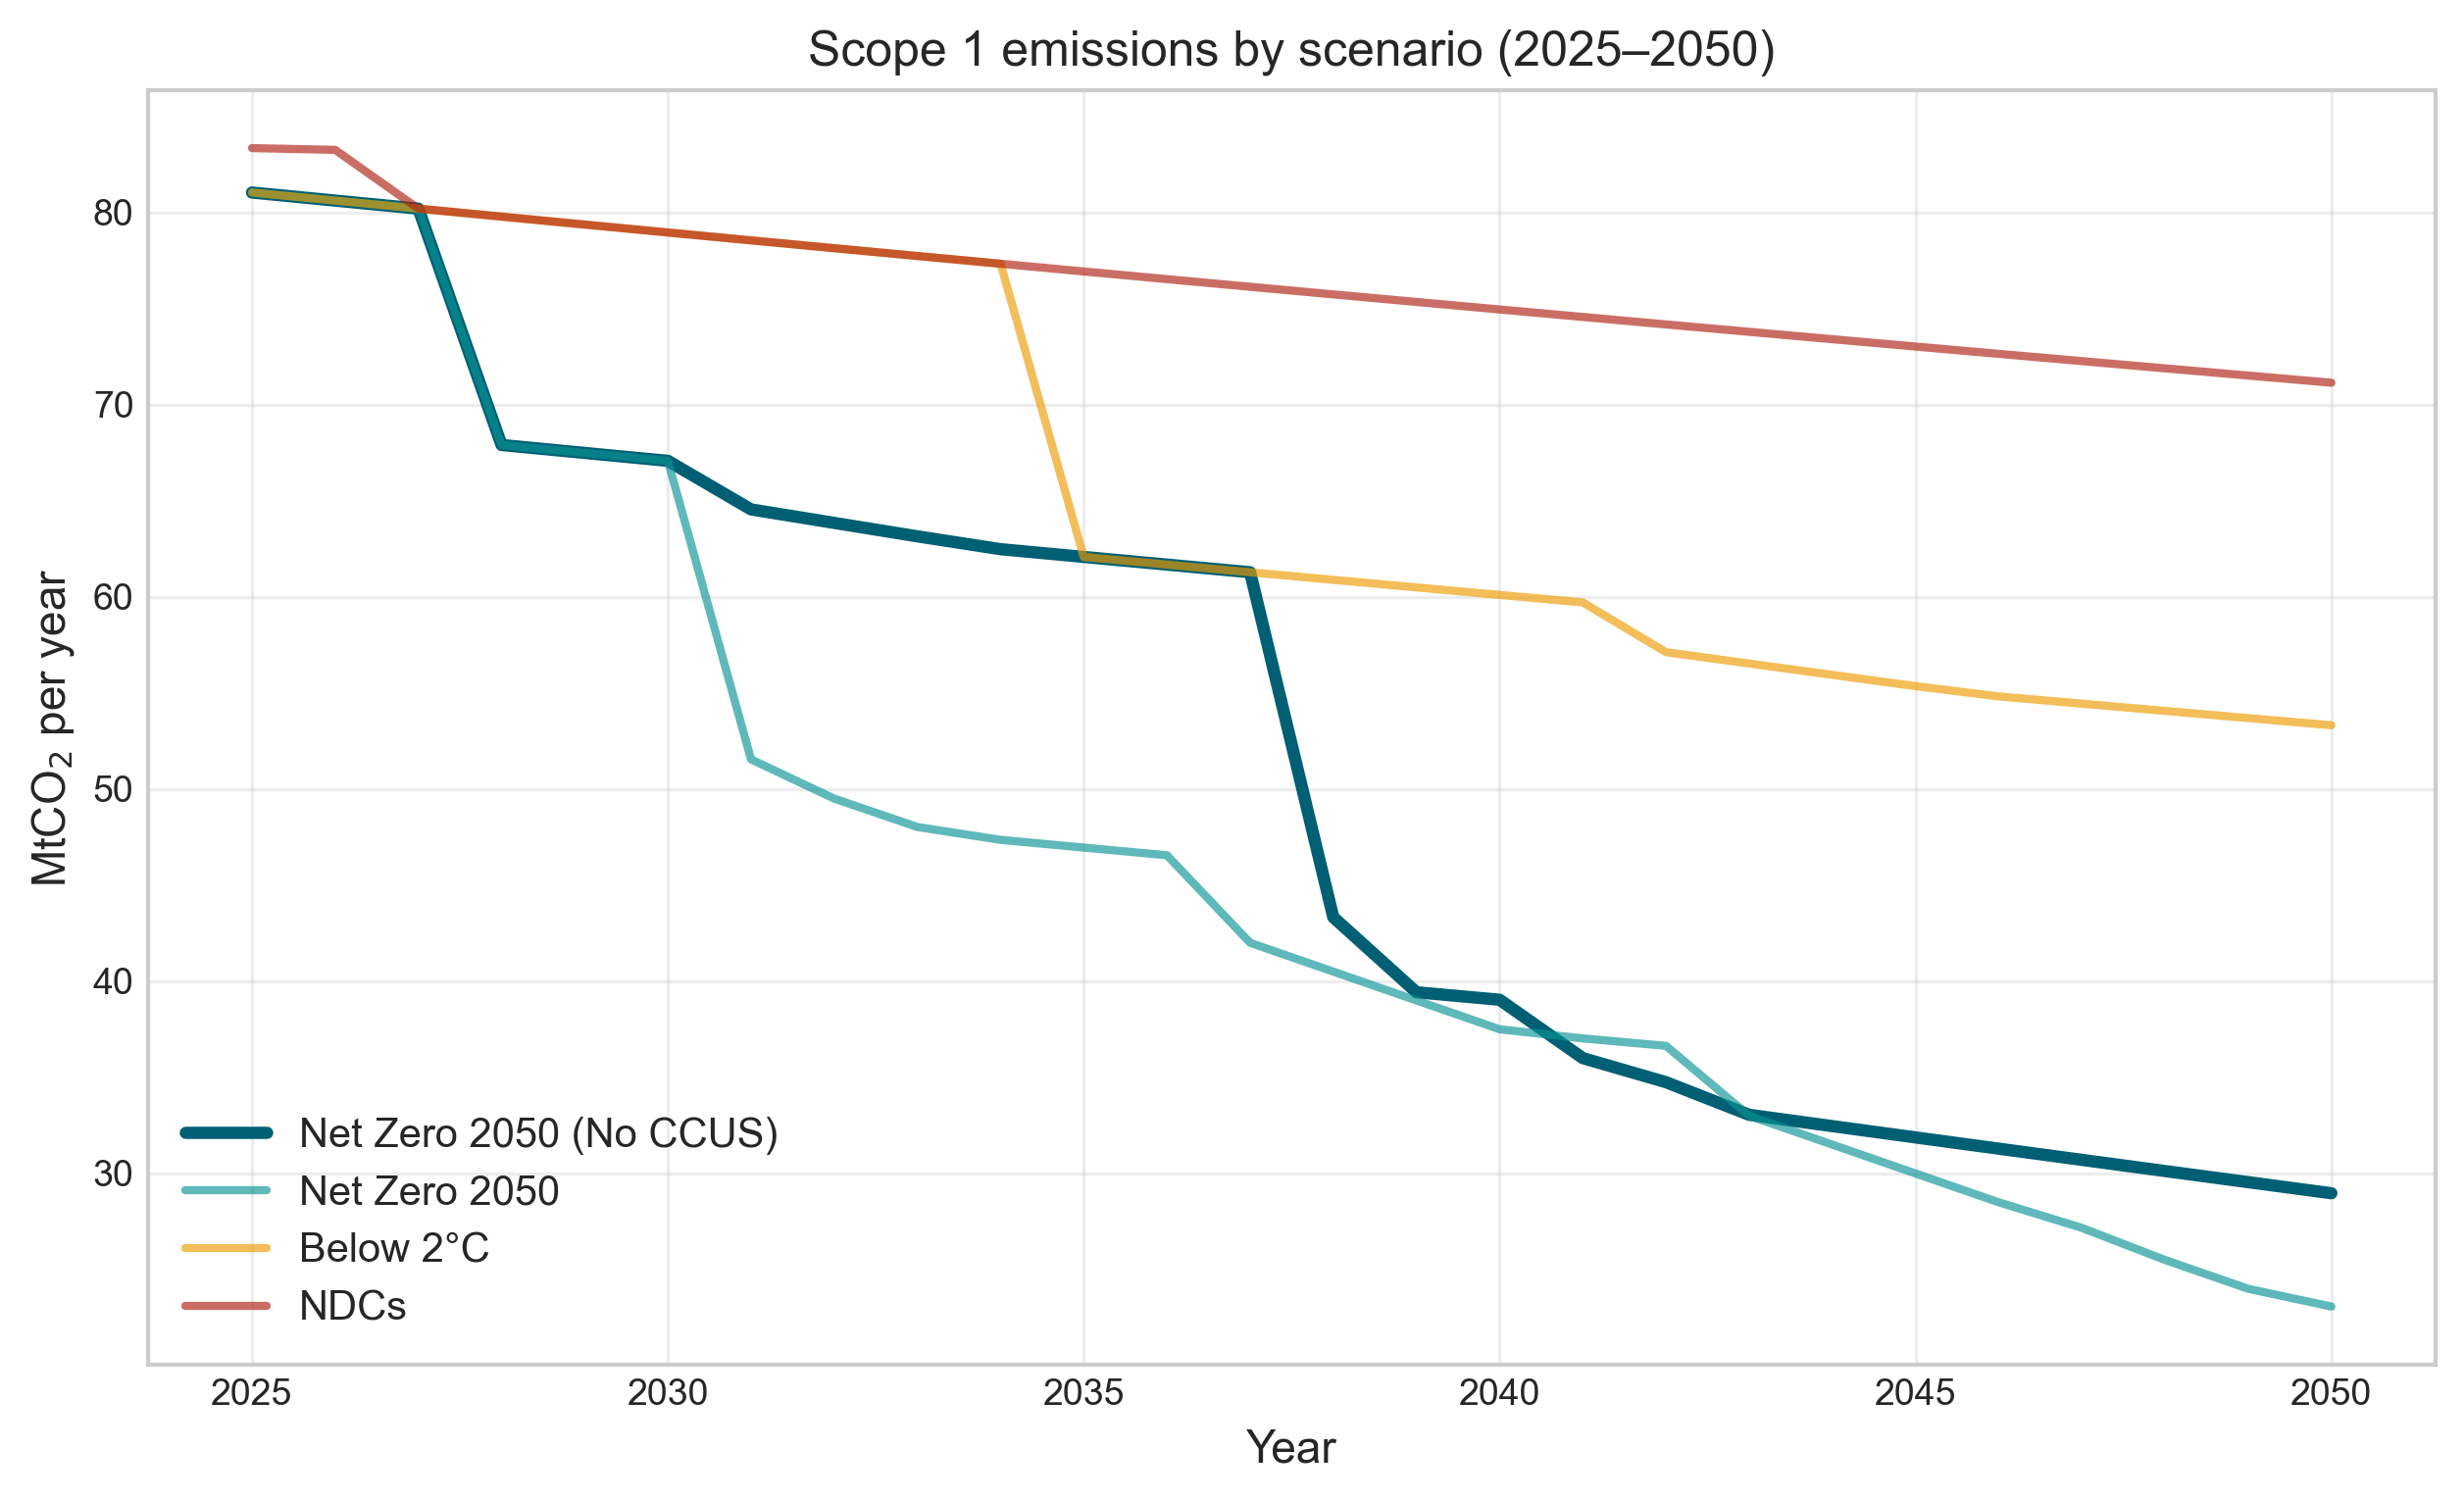
\includegraphics[width=0.8\linewidth]{scope1_by_scenario}
  \caption{Scope~1 emissions by scenario, including the Net Zero 2050 pathway with CCUS disabled (2025--2050).}
  \label{fig:scope1-by-scenario}
\end{figure}

These reductions matter enormously—the difference between NDC pricing and Net Zero pricing amounts to 791 MtCO$_2$ of avoided emissions over the planning horizon. Yet as we show in Section 4.3, even the most ambitious scenario still overshoots POSCO's allocated carbon budget. The price sensitivity is clear, but absolute price levels remain inadequate.

The No CCUS sensitivity reveals how dependent these pathways are on carbon capture technology. Removing CCUS availability while maintaining the same Net Zero price trajectory leaves emissions "stuck" above 45 MtCO$_2$ through the 2030s, declining only gradually to 29 MtCO$_2$ by 2050. This 26\% higher endpoint compared to the CCUS-enabled case underscores that carbon pricing alone cannot drive sufficient emission reductions if key abatement technologies remain unavailable or uneconomic. The model finds alternative routes—particularly hydrogen DRI, as we detail below—but these prove more expensive and still fail to close the budget gap entirely.

\subsection{Technology transitions follow sharp price thresholds, not gradual shifts}

One of our most striking findings is how technology deployment responds to discrete price thresholds rather than gradual carbon price increases. The model's investment behavior exhibits threshold effects that have important implications for policy predictability and investment timing.

Figure~\ref{fig:technology-transition} and Table~\ref{tab:annual-shares-ngfs_netzero2050} show that scrap-based EAF deployment remains essentially frozen—locked at just 4.5\% of total output—while carbon prices stay below \$100/tCO$_2$. Then, once the Net Zero pathway crosses \$110/tCO$_2$ in 2028, scrap-EAF share jumps suddenly to 22.8\% as the model builds a single 9 Mt capacity tranche. This discrete jump reflects the lumpy nature of steel industry investment: POSCO cannot gradually expand scrap-EAF capacity because it must construct entirely new facilities from scratch. The company's current operations are almost exclusively blast-furnace based, with only 1.7 Mt/y of specialty stainless EAF assets that cannot substitute for automotive-grade flat products \citep{POSCO2023SR}. Building EAF capacity means greenfield investment in complete production modules.

\begin{figure}[!t]
  \centering
  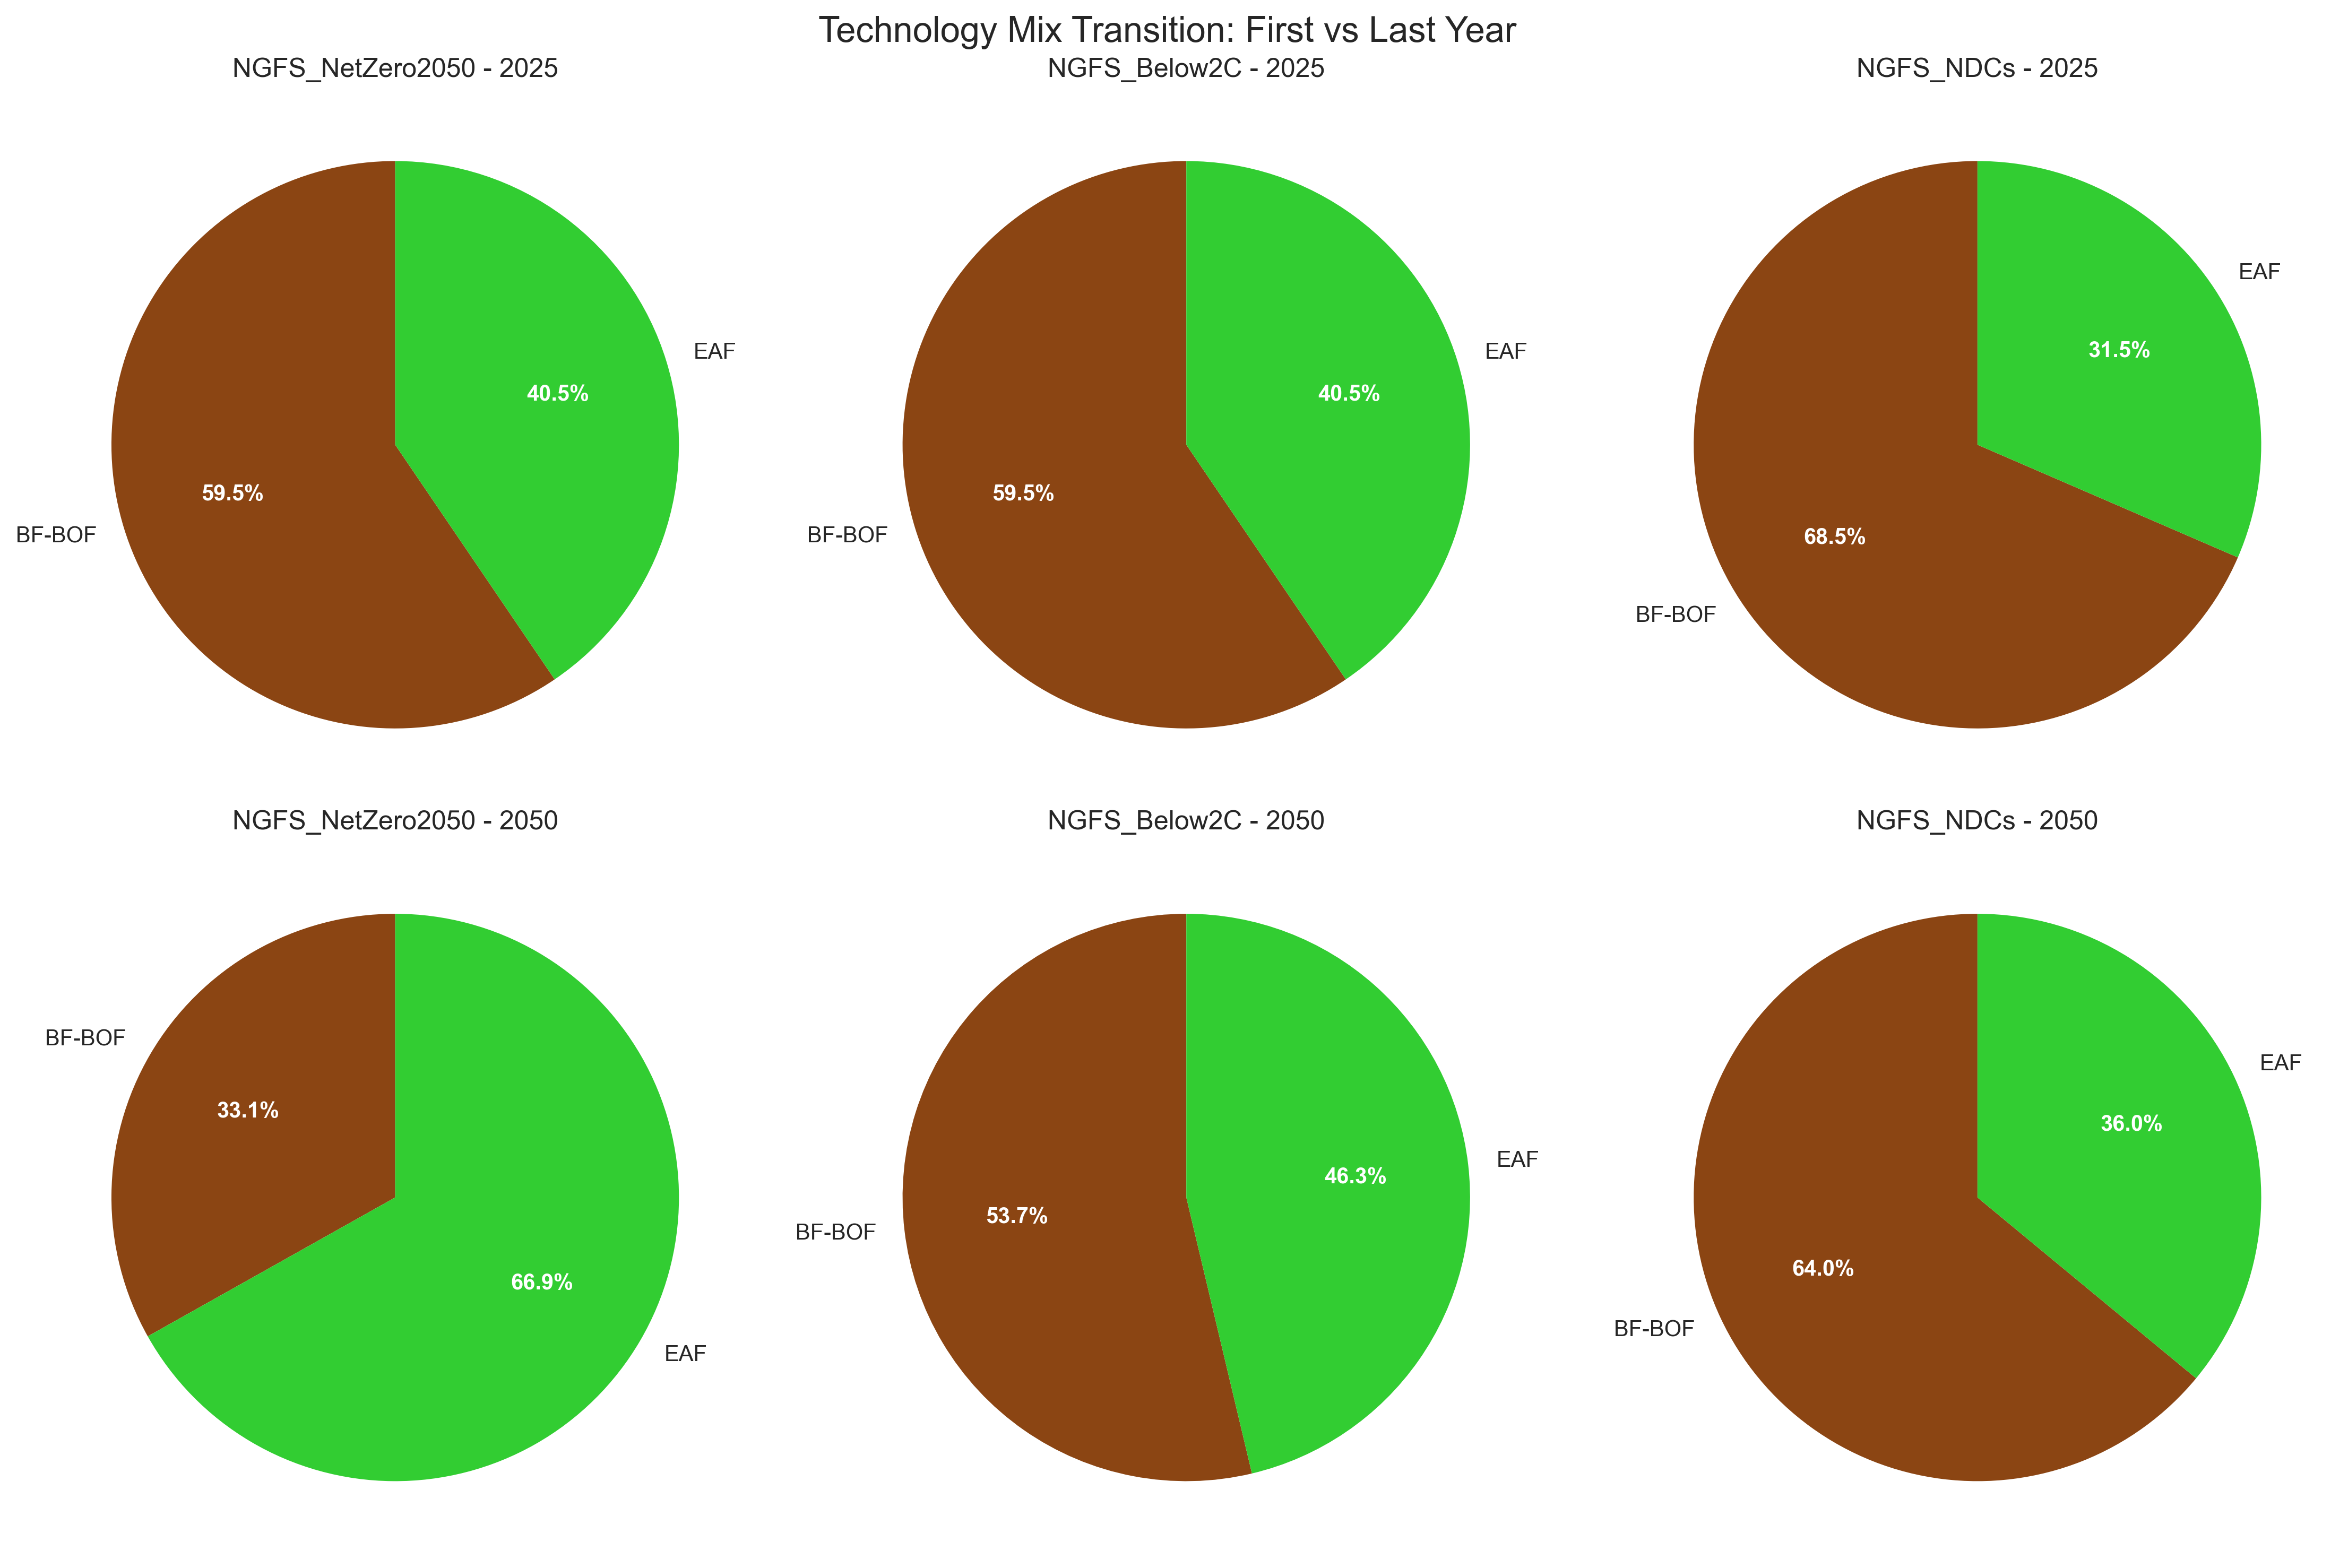
\includegraphics[width=0.8\linewidth]{technology_transition}
  \caption{Technology shares by scenario. The top panel emphasizes the Net Zero 2050 pathway with CCUS disabled; lower panels show the NGFS Net Zero, Below~2$^\circ$C, and NDC trajectories.}
  \label{fig:technology-transition}
\end{figure}

\begin{figure}[!t]
  \centering
  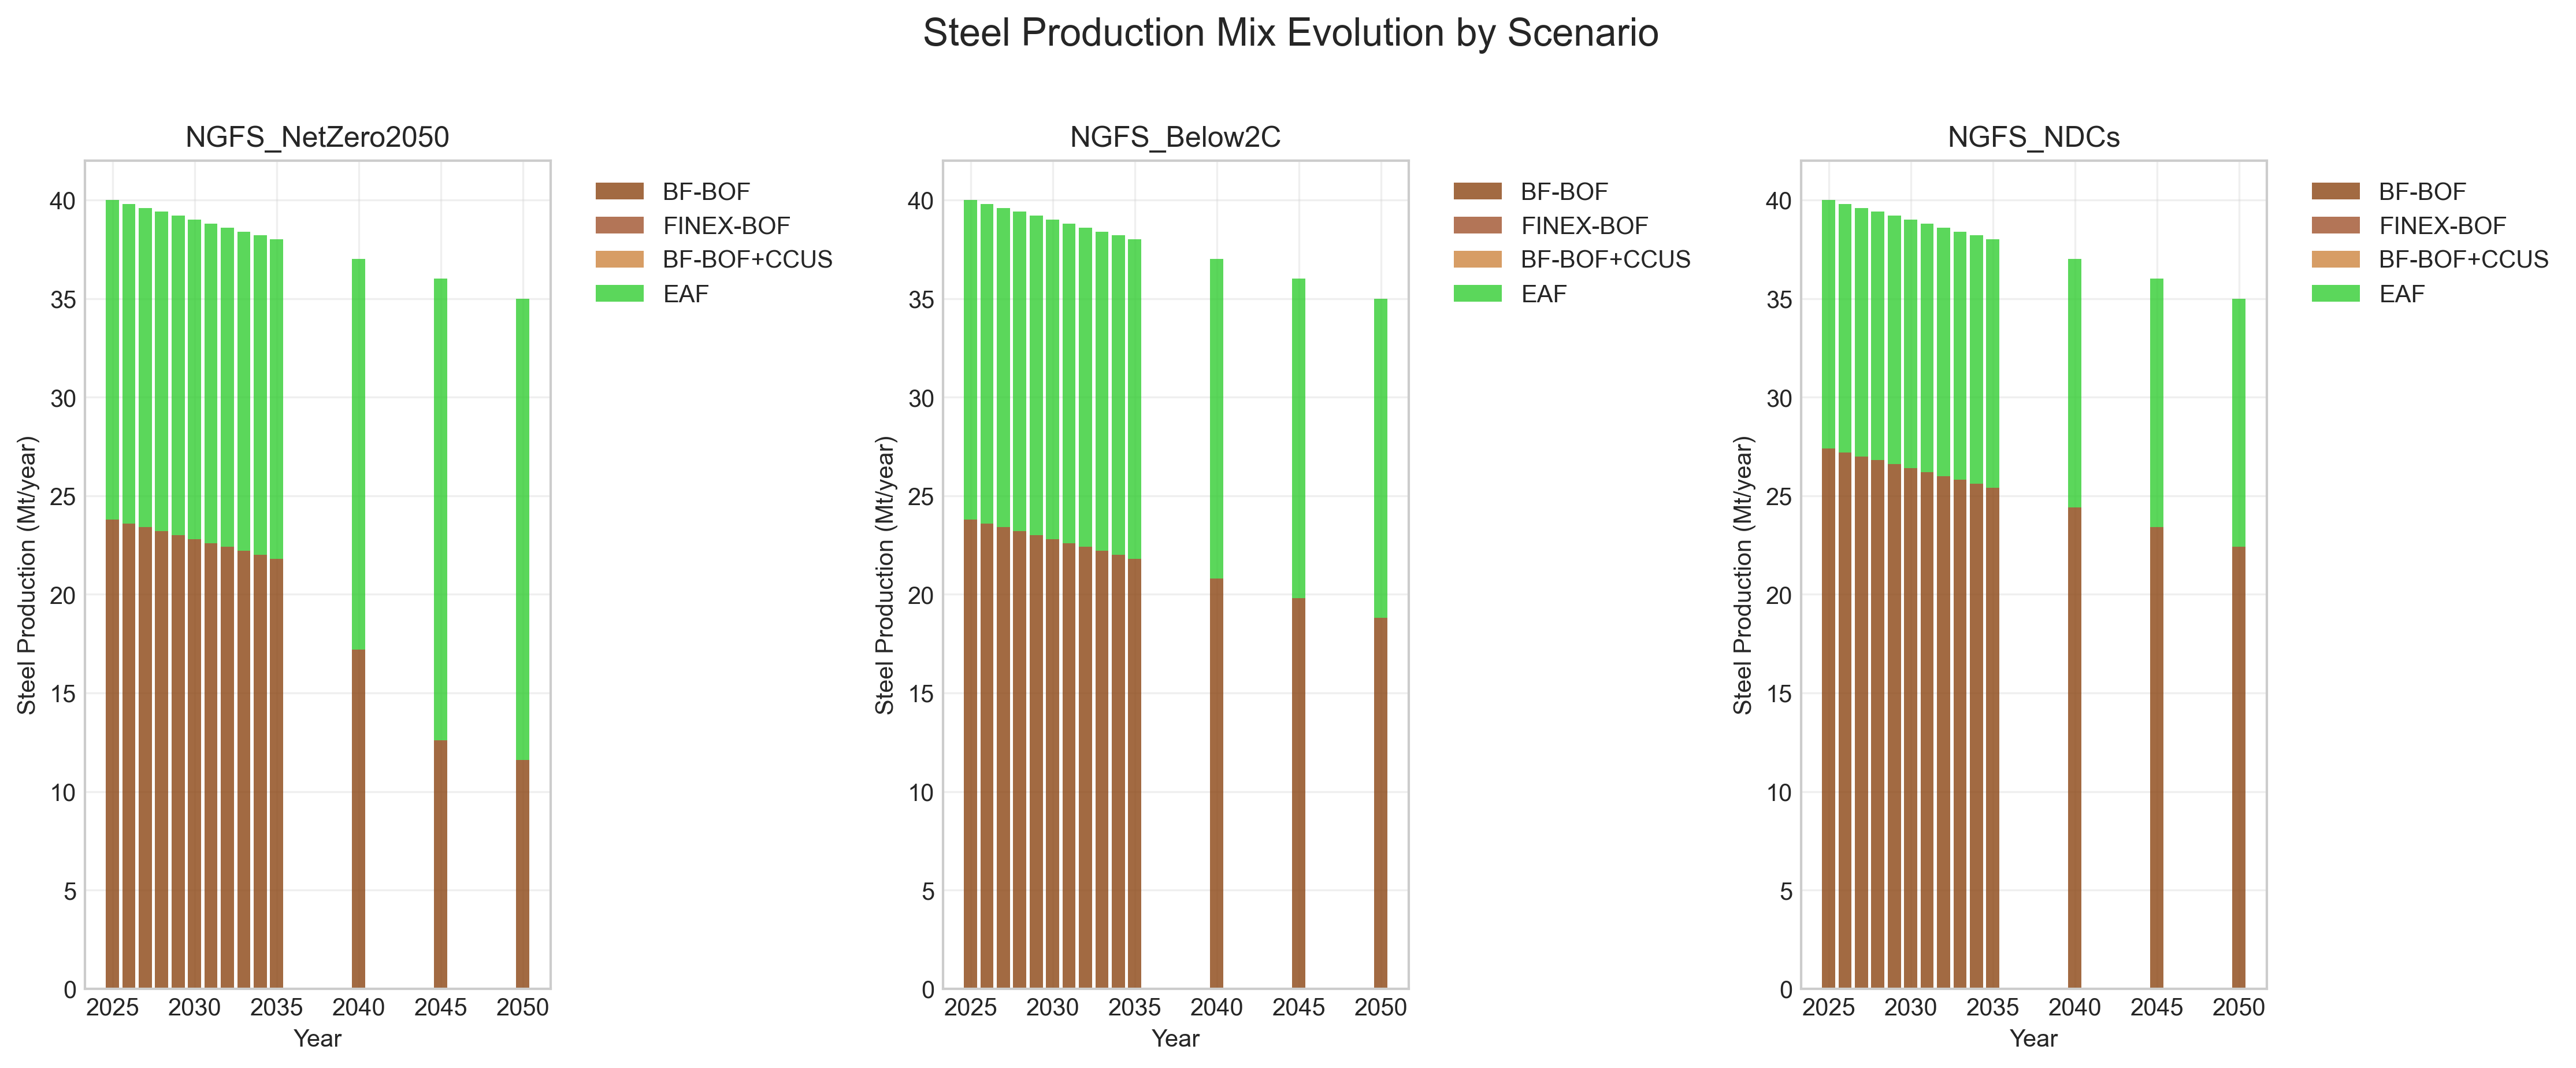
\includegraphics[width=0.8\linewidth]{production_mix_evolution}
  \caption{Production mix by technology route (Mt/year). Panels mirror Figure~\ref{fig:technology-transition}, with the Net Zero 2050 (No CCUS) case highlighted.}
  \label{fig:production-mix}
\end{figure}

Scrap availability then caps further EAF expansion at 35.7\% of output even under the most aggressive carbon prices. This ceiling reflects Korea's structural scrap deficit—unlike scrap-rich markets such as the United States, Korea must import substantial quantities of high-quality scrap to supply EAF operations. The binding constraint is not capital cost or carbon price, but physical feedstock availability.

Carbon capture exhibits similar threshold behavior but at even higher price levels. CCUS retrofits enter the portfolio only after carbon prices reach \$165/tCO$_2$ in 2031. At that point, the model retrofits one 9 Mt blast furnace module with capture equipment. Subsequent price increases to \$225/tCO$_2$ and \$255/tCO$_2$ trigger additional retrofits until CCUS-equipped furnaces supply 51\% of 2050 production under the Net Zero pathway. The economics are straightforward: CCUS retrofits carry a 65\% capital cost premium over conventional blast furnaces, requiring carbon prices above \$165/tCO$_2$ to justify the investment.

Lower price trajectories never activate carbon capture at all. The Below 2°C pathway peaks at \$240/tCO$_2$—high, but not quite high enough to justify widespread CCUS deployment. As a result, 64\% of output in 2050 remains unabated blast furnaces under this scenario. The NDC ceiling of \$100/tCO$_2$ fails to justify any structural technology change, keeping the BF-BOF share above 95\% throughout the entire planning horizon (see Tables~\ref{tab:annual-shares-ngfs_below2c} and \ref{tab:annual-shares-ngfs_ndcs}).

The policy implication is clear: if policymakers want to trigger low-carbon technology deployment, they need carbon prices sustained well above \$150/tCO$_2$—not just peak prices, but sustained multi-decade trajectories. Gradual price increases that never cross critical thresholds will not drive transformation.

Perhaps most revealing is what the model does not choose. Hydrogen-based direct reduction, natural gas DRI, and POSCO's proprietary FINEX technology remain dormant across all scenarios, even at carbon prices reaching \$450/tCO$_2$. The reason is straightforward: at our baseline hydrogen cost assumptions (\$4.5/kg in 2030, declining to \$2.5/kg by 2050), hydrogen routes simply cannot compete economically with the CCUS-plus-scrap combination. Our cost assumptions align with major techno-economic assessments \citep{MaterialEconomics2019,demailly2018european}, which estimate that hydrogen steel requires delivered hydrogen below \$2.0-2.5/kg to reach cost parity with conventional routes—a threshold our baseline trajectory barely approaches by 2050.

This finding challenges narratives that position hydrogen as the primary decarbonization pathway for steel. Under realistic cost assumptions and within the 2025-2050 timeframe, carbon pricing alone cannot make hydrogen competitive. Only when we disable CCUS entirely (discussed in Section 4.6) does the model reluctantly turn to hydrogen DRI—and even then, the outcome is worse on both emissions and costs.

\subsection{All carbon price trajectories overshoot the sectoral budget—even Net Zero}

We now confront the central research question: can carbon pricing drive investment decisions that remain within climate-consistent carbon budgets? The answer is unequivocal: no. Figure~\ref{fig:emissions-pathways} and our cumulative emission calculations reveal systematic budget overshoots across all scenarios.

\begin{figure}[!t]
  \centering
  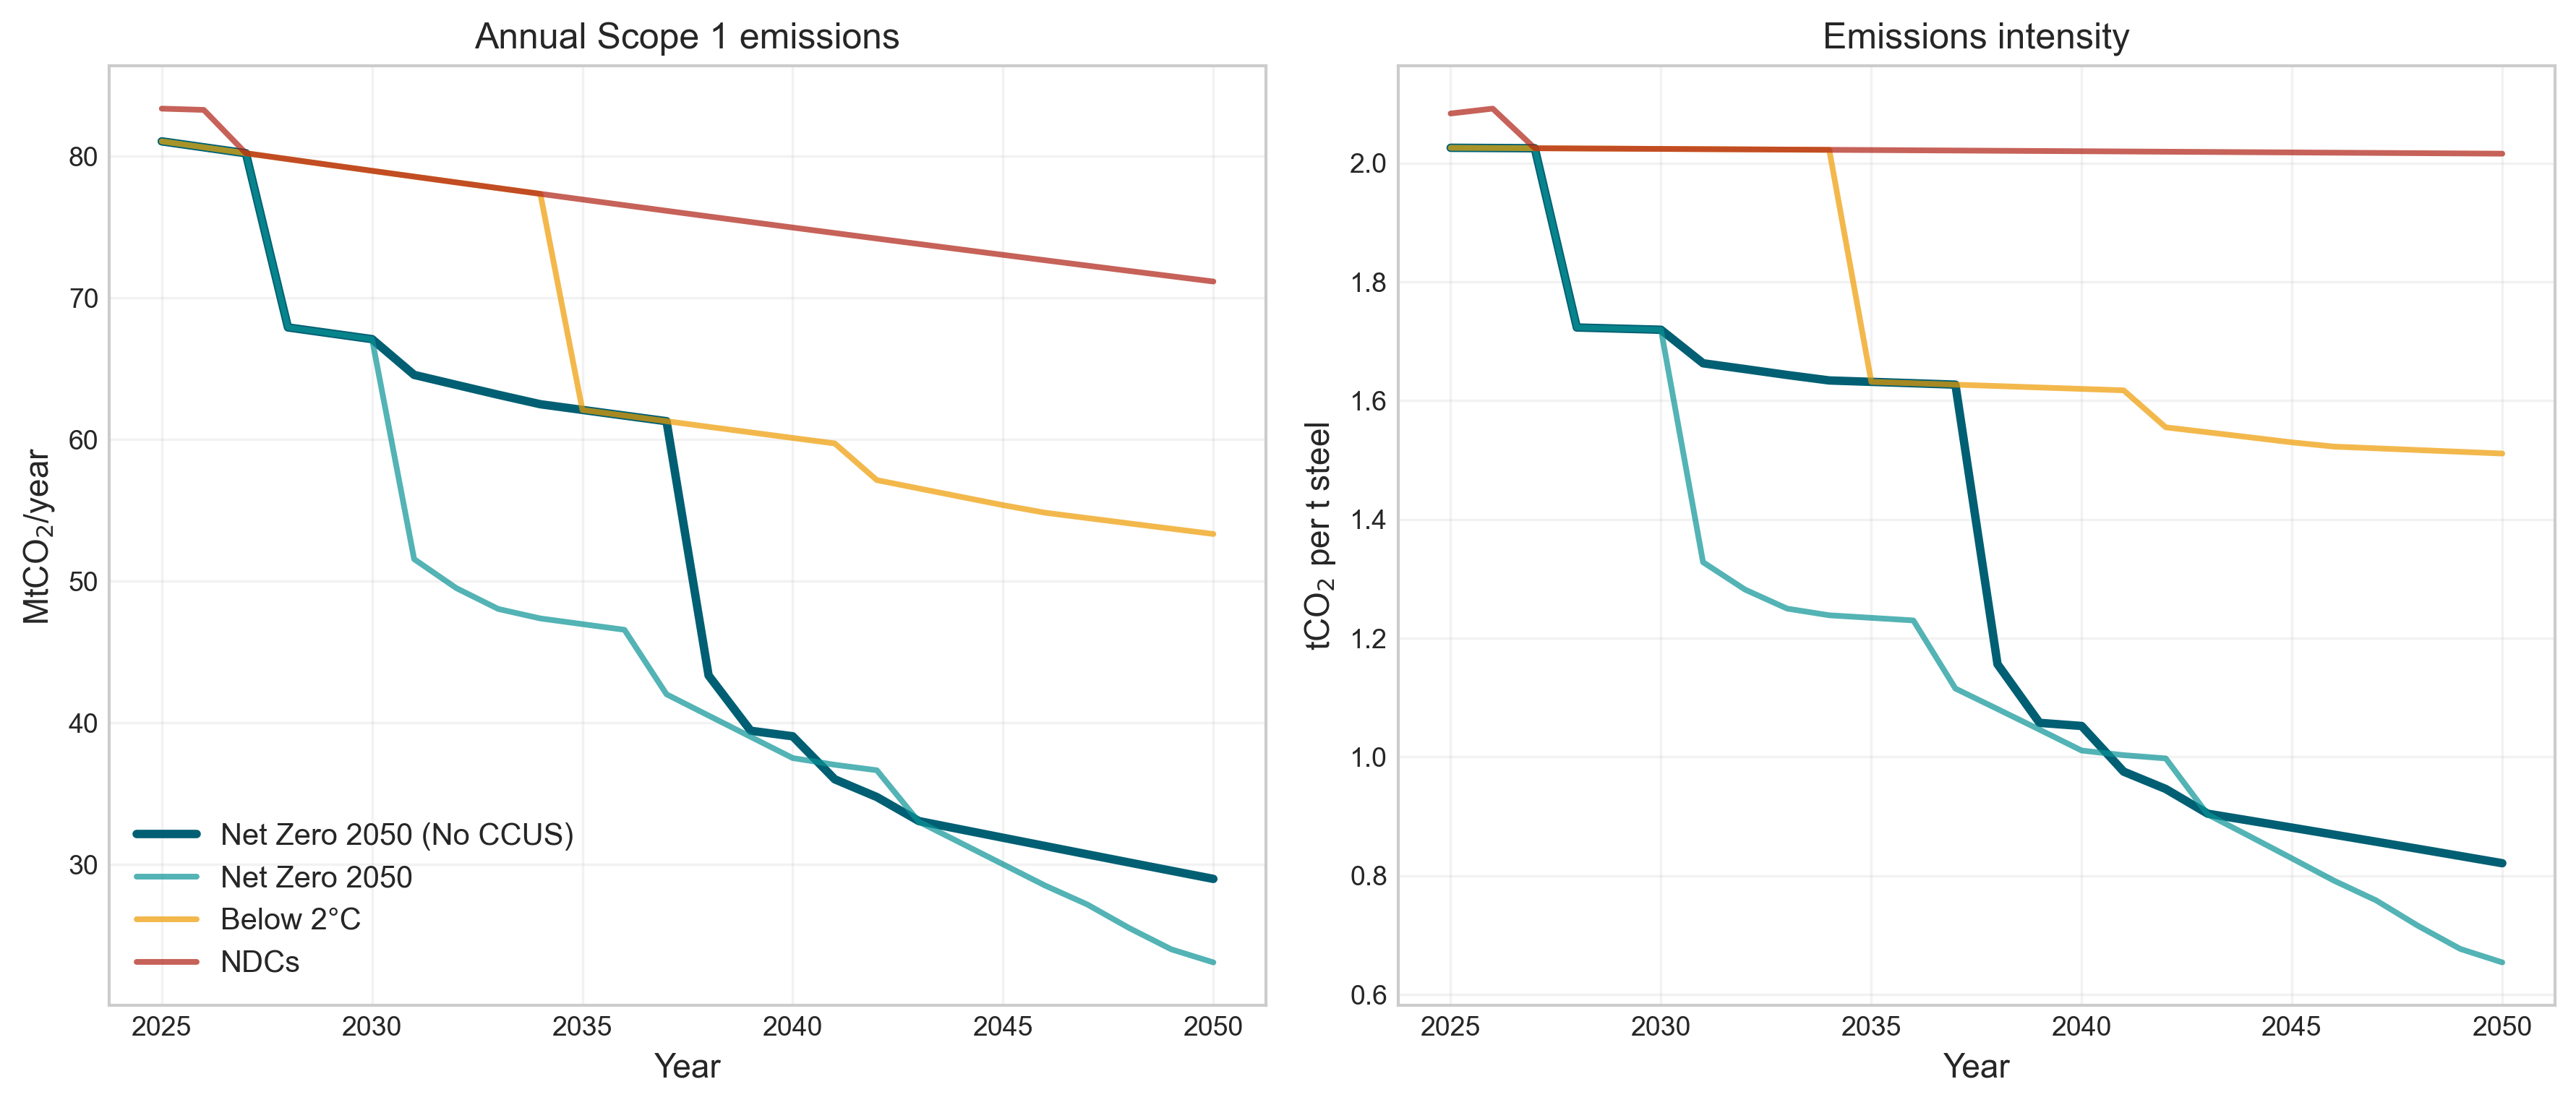
\includegraphics[width=0.85\linewidth]{emissions_pathways}
  \caption{Annual Scope~1 emissions (left) and emissions intensity (right) by scenario.}
  \label{fig:emissions-pathways}
\end{figure}

Integrating annual emissions over the 2025-2050 period produces cumulative totals of 1,190 MtCO$_2$ under Net Zero pricing, 1,713 MtCO$_2$ under Below 2°C, and 1,981 MtCO$_2$ in the NDC case. Compared with POSCO's allocated carbon budget of 1,110 MtCO$_2$ (derived in Section 3.3), the overshoots are:

\begin{itemize}[leftmargin=*]
  \item \textbf{Net Zero 2050:} +80 MtCO$_2$ (+7.2\%)
  \item \textbf{Below 2°C:} +603 MtCO$_2$ (+54\%)
  \item \textbf{NDCs:} +871 MtCO$_2$ (+78\%)
\end{itemize}

Let us put these numbers in perspective. The Below 2°C overshoot of 603 MtCO$_2$ represents more than half the entire allocated budget—POSCO would need to cut an additional 35\% from its optimized emission pathway to achieve compliance. The NDC overshoot of 871 MtCO$_2$ is simply catastrophic from a climate perspective, representing nearly 80\% excess emissions above the budget.

Even the most ambitious Net Zero scenario overshoots by 80 MtCO$_2$, or 7.2\%. This residual gap is particularly revealing because it persists despite carbon prices reaching \$450/tCO$_2$ by 2050—levels far beyond anything currently implemented in carbon markets globally. The implication is that budget compliance would require either carbon prices rising well above \$450/tCO$_2$ in later periods, or complementary policies that constrain production or mandate specific technologies beyond what price signals alone can deliver.

The cumulative gap maps directly onto a carbon price gap. Moving from the NDC ceiling (\$100/tCO$_2$) to the Net Zero peak (\$450/tCO$_2$) yields a 791 MtCO$_2$ reduction—implying that each additional \$100/tCO$_2$ of carbon price drives roughly 226 MtCO$_2$ of cumulative abatement over the planning horizon. The residual 80 MtCO$_2$ shortfall under Net Zero would require sustained prices above \$500/tCO$_2$ to close entirely through carbon pricing alone.

Free allocation exacerbates this problem substantially. Even under the Net Zero pathway, only 72 MtCO$_2$ of cumulative emissions face actual ETS liability—just 6\% of total emissions. The Below 2°C pathway pays for only 596 MtCO$_2$ out of 1,713 MtCO$_2$ emitted (35\%), while the NDC case sees 863 MtCO$_2$ of net ETS-liable emissions (44\%). This means that most emissions remain effectively unpriced despite rising nominal carbon prices, because free allocation shields firms from marginal carbon costs.

Closing the residual budget gap under Net Zero therefore requires one of two interventions: either a sharper price floor escalation after 2040 that drives prices well above \$500/tCO$_2$, or a much faster phase-down of free allocation so that firms internalize full carbon costs before the next blast furnace relining cycle in the early 2030s. Without addressing free allocation, even extremely high nominal carbon prices will continue to undershoot climate targets. Detailed budget compliance calculations are provided in the supplementary data file \texttt{outputs/analysis/carbon\_budget\_compliance.csv}.

Figure~\ref{fig:emissions-pathways} shows that only the NGFS Net Zero pathways materially shift emissions intensity below 1.0 tCO$_2$/t steel by 2050. The No CCUS sensitivity keeps intensity stubbornly above 0.8 tCO$_2$/t even in 2050, reflecting continued reliance on hydrogen DRI and residual unabated blast furnaces. This emissions intensity comparison reinforces that transforming the steel sector requires not just incremental improvements but wholesale technology replacement—exactly the kind of lumpy, expensive transitions that carbon pricing struggles to trigger without extremely high and sustained price signals.

\subsection{Higher carbon prices reduce total costs by substituting capital for compliance}

A counterintuitive but important finding emerges when we examine total system costs: more ambitious carbon pricing actually lowers lifetime costs rather than raising them. This result challenges common industry narratives that higher carbon prices necessarily harm competitiveness and profitability.

Summing undiscounted expenditure over the entire 2025-2050 period, the Net Zero pathway delivers the lowest lifetime system cost at \$791 billion, compared to \$871 billion for Below 2°C and \$842 billion for the NDC case. Dividing by cumulative steel output (978 Mt over the period) yields average costs of \$810/t under Net Zero, \$891/t under Below 2°C, and \$861/t in the NDC scenario.

At first glance, this seems paradoxical—how can higher carbon prices reduce costs? The mechanism is straightforward: ambitious pricing allows firms to substitute upfront capital investment in low-carbon technologies for recurring carbon compliance payments. Under the NDC trajectory, carbon prices remain low (\$100/tCO$_2$ ceiling), which means technologies like CCUS never become cost-justified. The firm therefore continues operating conventional blast furnaces and pays recurring ETS fees year after year. These compliance costs accumulate to \$59.7 billion over the planning horizon, representing 7.1\% of lifetime expenditure.

By contrast, Net Zero pricing justifies major CCUS retrofits and scrap-EAF expansion in the 2030s. While these investments carry high upfront capital costs, they dramatically reduce ongoing carbon liabilities. Total emissions under Net Zero reach 1,190 MtCO$_2$, but only 72 MtCO$_2$ face ETS liability after accounting for free allocation. This trims total compliance payments to just \$9.3 billion—merely 1.2\% of lifetime costs. The firm redirects cash flow from recurring carbon fees toward productive capital investment that permanently lowers emissions.

Table~\ref{tab:cost-abatement} quantifies this trade-off using marginal abatement cost metrics. Moving from the NDC baseline to Net Zero actually shows negative abatement costs of \$64/tCO$_2$—meaning the firm saves money while reducing emissions. The intermediate Below 2°C pathway requires positive \$108/tCO$_2$ in incremental support because carbon prices peak too early (\$240/tCO$_2$) to justify full CCUS deployment, leaving the firm in an awkward middle ground where it invests in partial decarbonization but still pays substantial carbon fees.

\begin{figure}[!t]
  \centering
  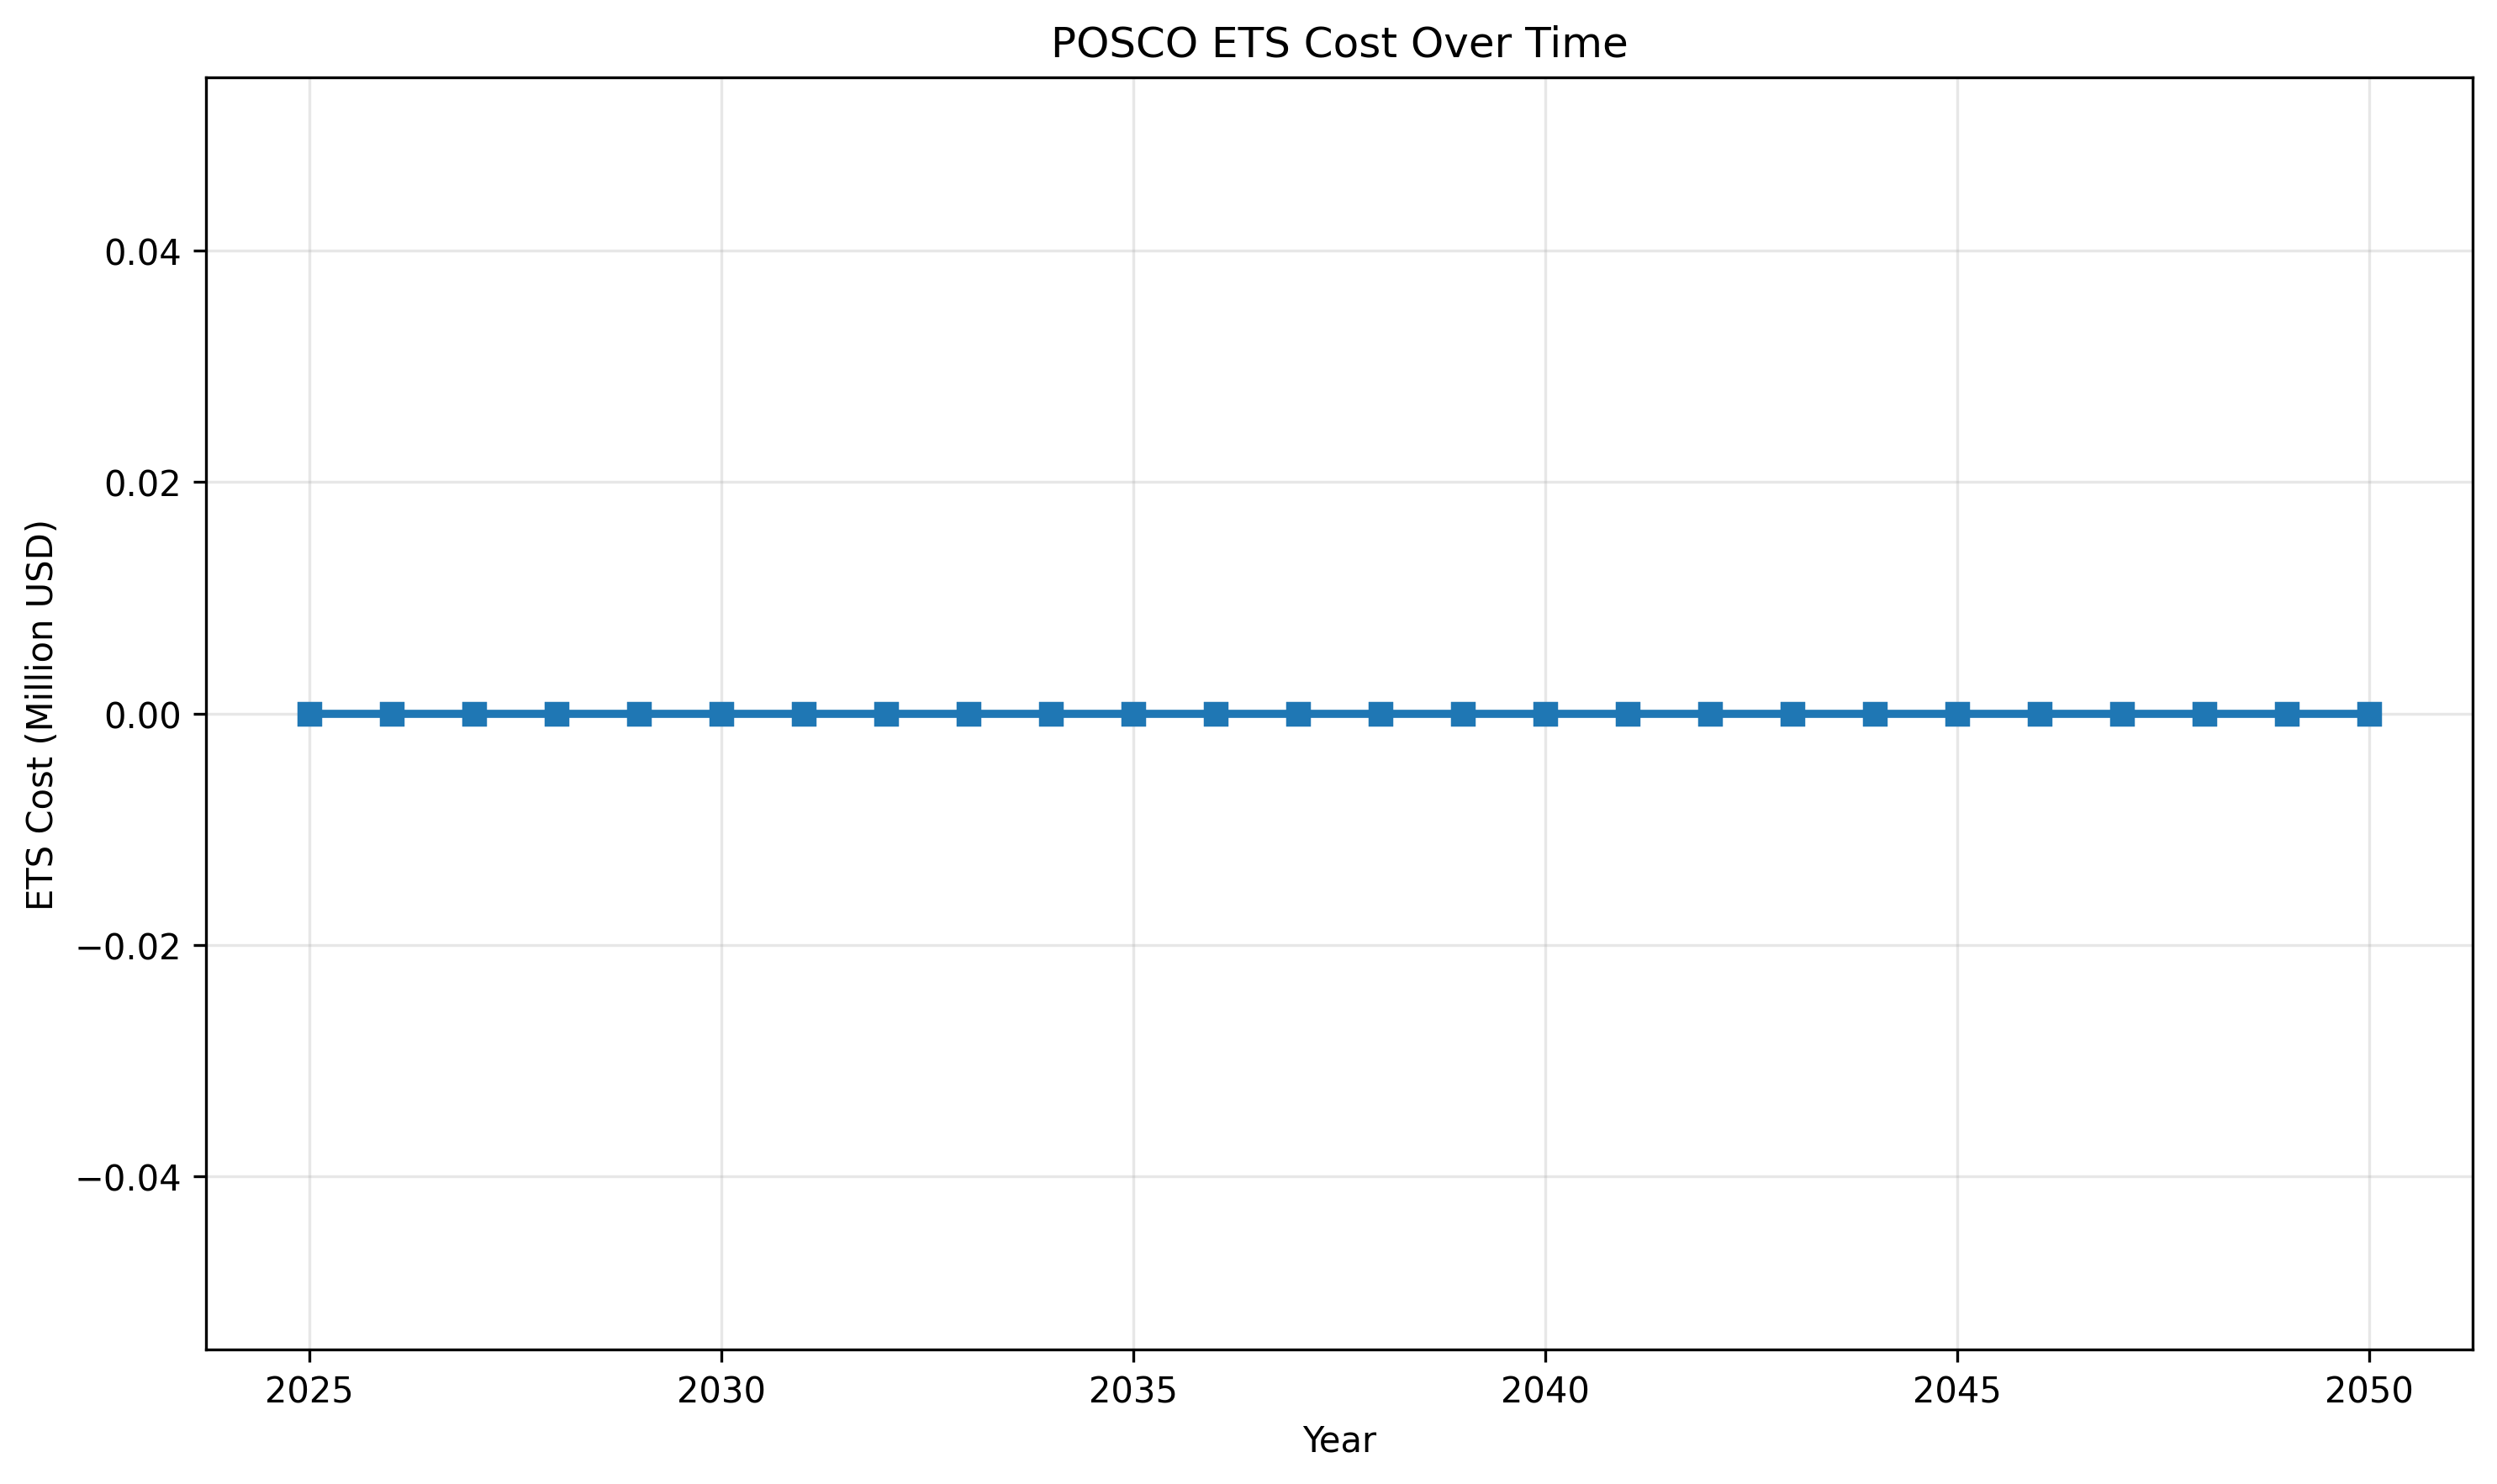
\includegraphics[width=0.8\linewidth]{ets_cost_by_scenario}
  \caption{Annual ETS compliance costs across the NGFS price trajectories plus the Net Zero 2050 (No CCUS) sensitivity.}
  \label{fig:ets-costs}
\end{figure}

Figure~\ref{fig:ets-costs} visualizes how compliance payments evolve over time. The NDC scenario shows persistently high annual ETS costs through 2050, peaking above \$3 billion/year in the mid-2040s as emissions remain high while allowance prices gradually rise. Net Zero pricing shows a different pattern: modest compliance costs through the late 2020s while free allocation remains generous, then a spike in the early 2030s as allocation tightens before CCUS retrofits come online, and finally a collapse to near-zero costs post-2035 as low-carbon technologies dominate the portfolio.

The policy implication is powerful: ambitious carbon pricing need not harm industrial competitiveness if it reaches levels sufficient to justify transformative investment. Half-measures that raise carbon prices modestly without crossing technology deployment thresholds create the worst of both worlds—firms face rising compliance costs without the price certainty needed to justify major capital commitments.

\subsection{CCUS unavailability quadruples carbon costs and forces expensive hydrogen adoption}

To test how critically our results depend on CCUS availability, we re-run the Net Zero 2050 price trajectory with carbon capture technology completely disabled (setting capture efficiency to zero). This sensitivity reveals stark trade-offs and highlights infrastructure dependencies that could derail decarbonization pathways.

Without CCUS, the technology portfolio shifts dramatically. Hydrogen-based direct reduction routes, which never appeared in the baseline scenarios, suddenly capture 35.7\% of production by 2050. Scrap-EAF remains capped at its feedstock-constrained maximum of 35.3\%, while unabated blast furnaces supply the remaining 29.0\% of output. The model has no choice but to turn to expensive hydrogen DRI because scrap availability is exhausted and conventional BF-BOF routes face prohibitive carbon costs without capture technology.

Yet the emission and cost outcomes deteriorate markedly compared to the CCUS-enabled pathway:

\begin{itemize}[leftmargin=*]
  \item Cumulative Scope 1 emissions climb to 1,324 MtCO$_2$, a +19\% increase versus the CCUS-enabled Net Zero case and a +19\% overshoot relative to the carbon budget.
  \item Annual emissions in 2050 settle at 29.0 MtCO$_2$, 26\% higher than the CCUS-enabled endpoint.
  \item Net ETS liabilities over the planning horizon jump from 72 MtCO$_2$ to 206 MtCO$_2$—nearly tripling.
  \item Cumulative ETS payments explode from \$9.3 billion to \$43 billion—more than quadrupling.
  \item Average steelmaking costs increase to \$815/t, eroding much of the competitiveness advantage delivered by CCUS-enabled pathways.
\end{itemize}

\begin{figure}[!t]
  \centering
  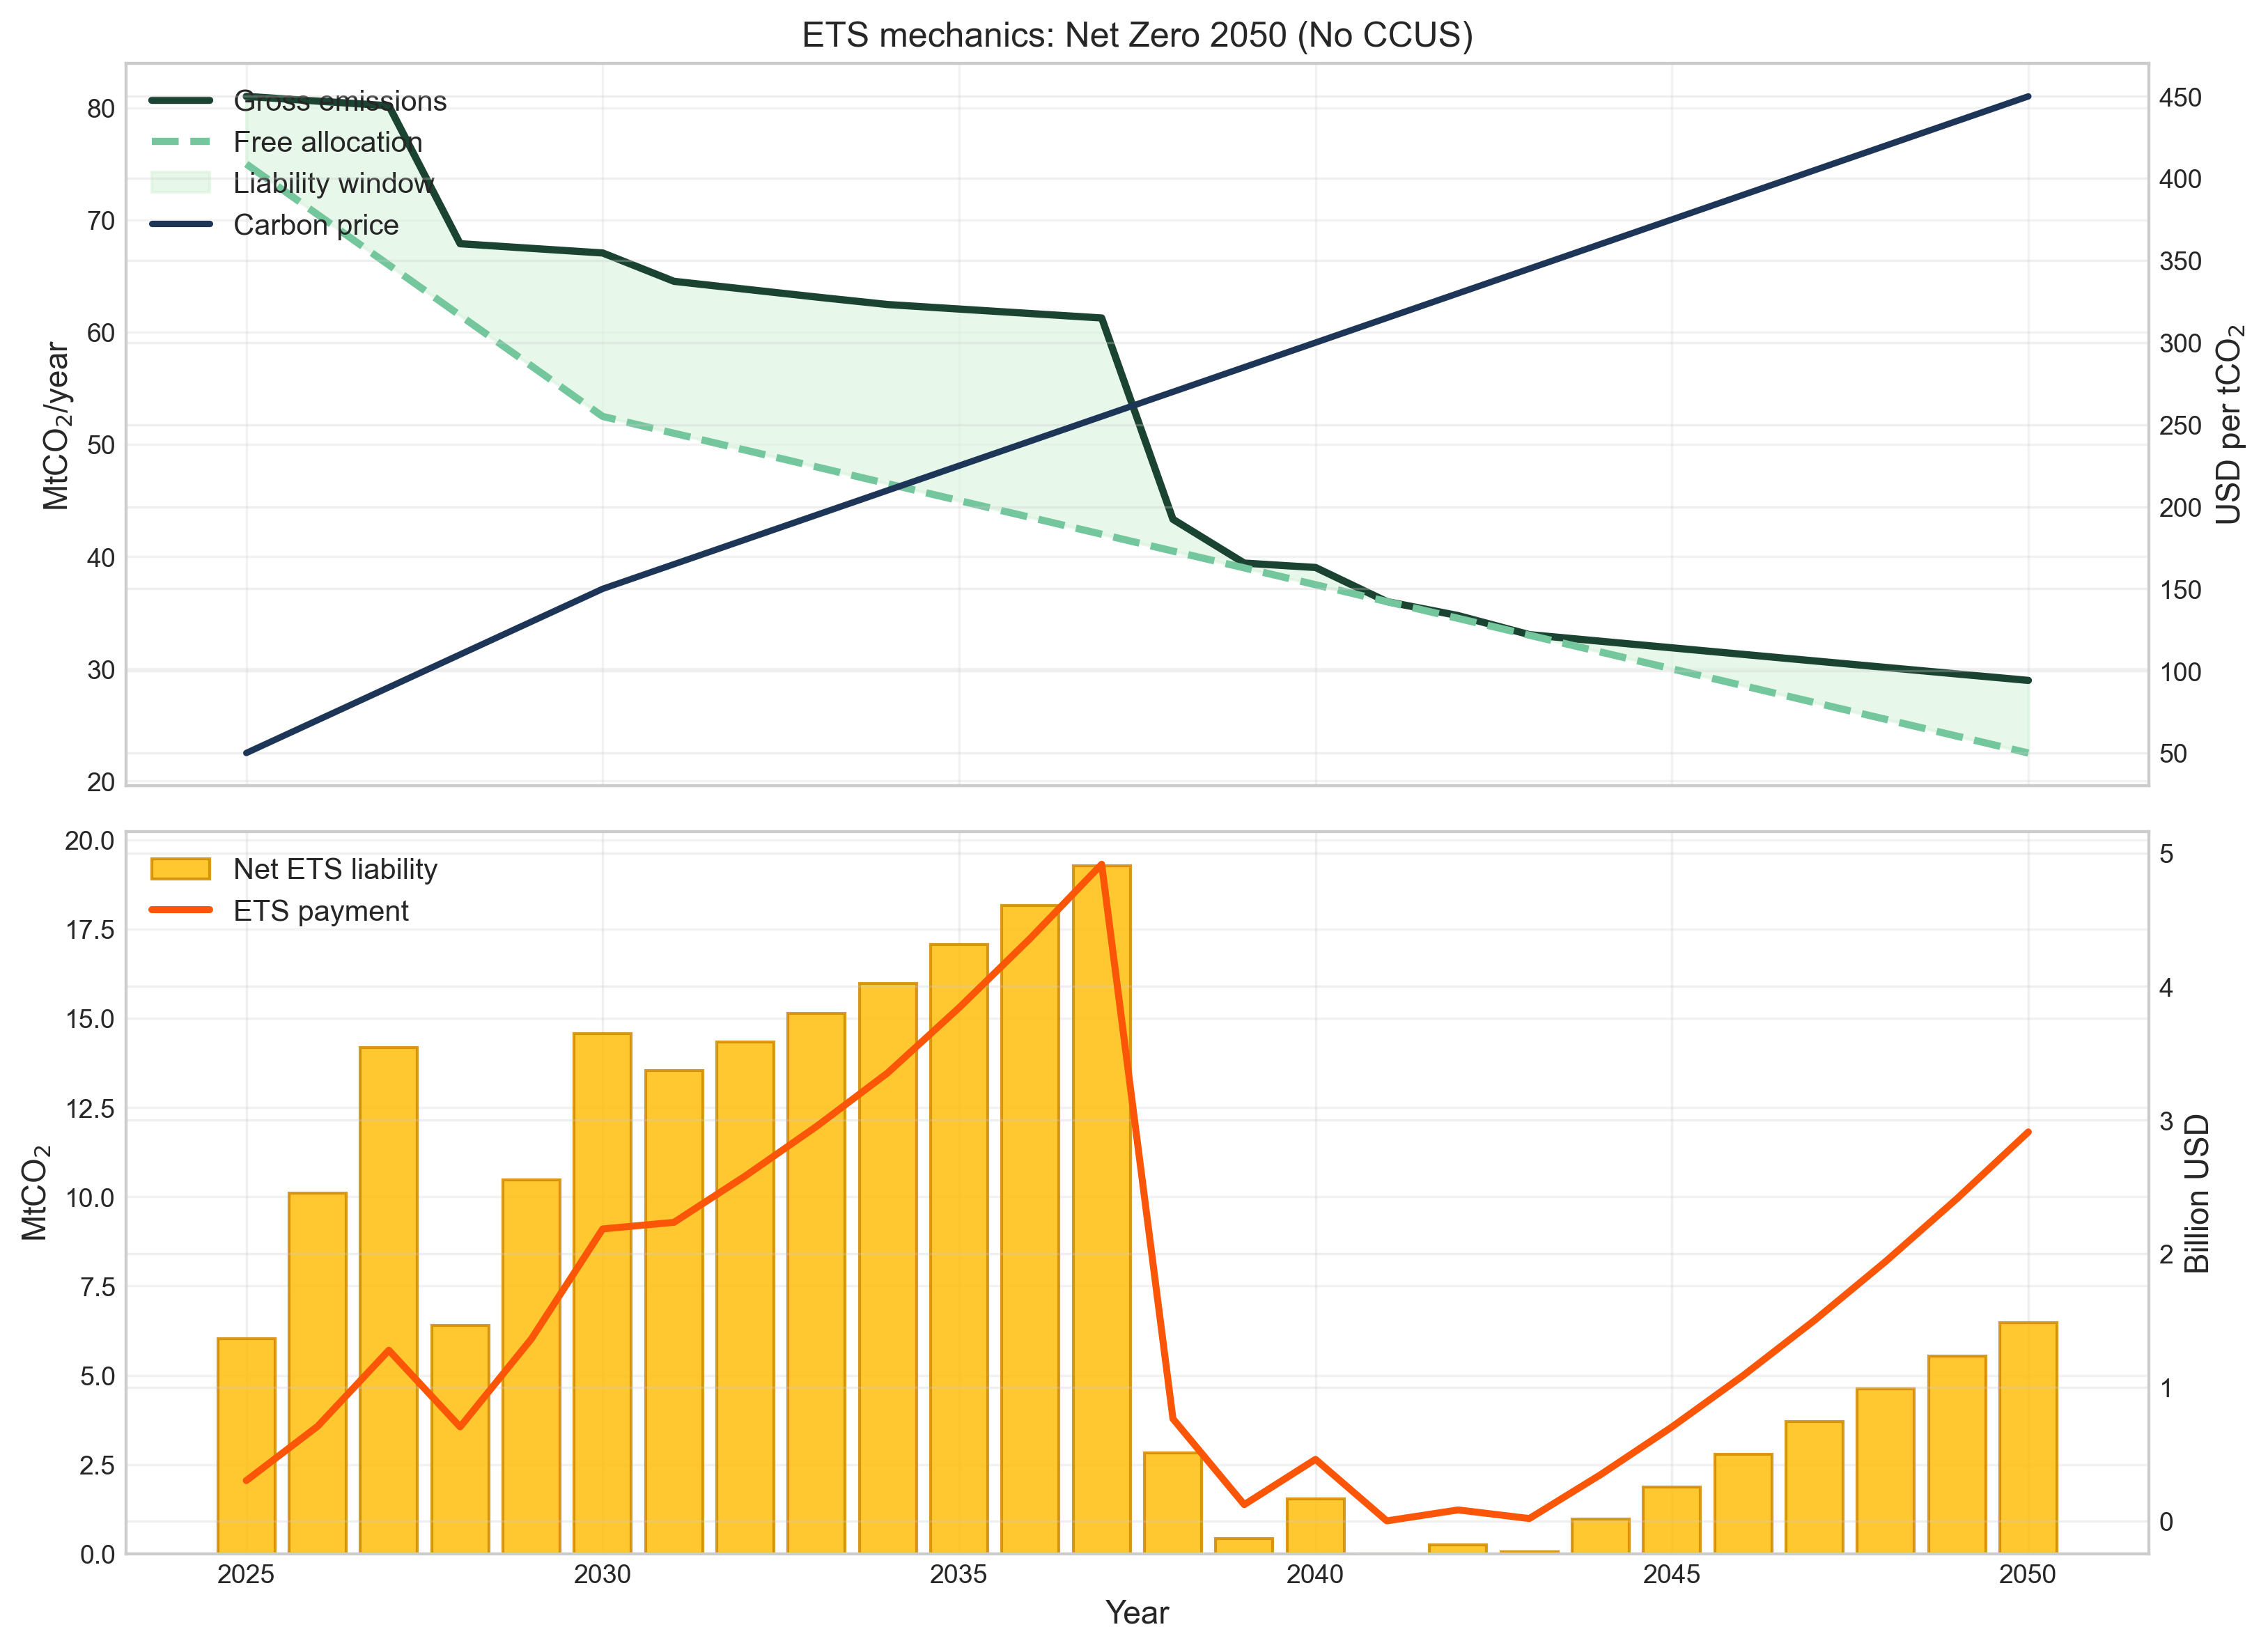
\includegraphics[width=0.85\linewidth]{ets_cost_logic}
  \caption{ETS cost mechanics for the Net Zero 2050 (No CCUS) pathway. The top panel contrasts gross emissions, free allocation, and allowance prices; the lower panel shows net ETS liabilities and resulting payments.}
  \label{fig:ets-logic}
\end{figure}

Figure~\ref{fig:ets-logic} illustrates the mechanism behind this cost explosion. The free allocation schedule declines steadily after 2030, but without CCUS technology to reduce gross emissions proportionally, a widening liability gap opens up. By the mid-2030s, net ETS liabilities exceed 5 MtCO$_2$/year. Combined with allowance prices crossing \$200-300/tCO$_2$, this generates multi-billion-dollar annual compliance payments that persist through 2050.

The No CCUS sensitivity underscores that hydrogen DRI adoption at current cost assumptions requires CCUS to absorb residual blast furnace output. Hydrogen alone cannot fully decarbonize the steel sector within realistic cost constraints—it needs CCUS as a complementary technology for transitional blast furnace operations. Without a credible CCUS program backed by CO$_2$ transport and storage infrastructure, the ETS would shoulder far larger compliance volumes, the carbon budget gap would remain unacceptably wide, and competitiveness would erode substantially.

This finding has crucial policy implications: Korea cannot simply choose between "green hydrogen" and "CCUS" as alternative decarbonization strategies. The cost-optimal pathway requires both—scrap-EAF where feedstock allows, CCUS retrofits for transitional blast furnace operations, and hydrogen DRI only for remaining capacity after exhausting cheaper options. Industrial policy that favors one technology over others risks missing this complementarity and driving suboptimal, expensive outcomes.

\subsection{Hydrogen cost breakthroughs alone cannot close the policy-performance gap}

To test whether lower hydrogen costs could fundamentally change technology choices and budget compliance, we conducted sensitivity analysis using alternative hydrogen price trajectories. The repository includes three scenarios (\texttt{outputs/h2\_breakthrough}, \texttt{h2\_optimistic}, and \texttt{h2\_zero}) that progressively reduce delivered hydrogen costs below our baseline assumptions.

The results are striking in their consistency. Even lowering hydrogen prices from the baseline \$4.5/kg to a "breakthrough" trajectory reaching \$2.5/kg by 2035—representing dramatic cost reductions from advanced electrolyzer deployment and cheap renewable electricity—barely shifts the technology mix under Net Zero pricing. Scrap-EAF rises modestly to 46\% of 2050 output (up from 36\% in baseline), CCUS-backed blast furnaces decline to 38\% (down from 51\%), and hydrogen DRI captures just 16\% of production rather than remaining at zero.

Cumulative emissions in this breakthrough hydrogen case reach 1,188 MtCO$_2$—essentially unchanged from the baseline 1,190 MtCO$_2$. Lifetime system costs shift by less than \$1.5 billion out of \$791 billion total, a rounding error. The carbon budget overshoot persists at +7.0\%, and policy implications remain identical.

We pushed this analysis to an extreme "zero-cost hydrogen" stress test where hydrogen is provided for free. Even under this utterly unrealistic assumption, cumulative emissions decline only to 1,175 MtCO$_2$—still overshooting the budget by +5.9\%. Why? Because capital intensity, ore quality constraints, and scrap availability ceilings—rather than hydrogen molecule prices alone—govern technology choices. Building hydrogen DRI facilities requires \$1,500/tpy in capital investment compared to \$800/tpy for conventional blast furnaces. Moreover, hydrogen DRI production requires high-quality direct-reduced iron pellets rather than standard iron ore fines, introducing feedstock constraints that limit hydrogen route expansion regardless of H$_2$ prices.

These sensitivities confirm that policy packages aimed solely at subsidizing hydrogen production would leave the carbon budget gap essentially intact unless paired with infrastructure investments that tackle non-price barriers: pellet production facilities for DRI feedstock, hydrogen pipeline networks and storage, and guaranteed off-take contracts that de-risk large capital commitments. The sobering conclusion is that simply making green hydrogen cheap will not transform the steel sector—the binding constraints lie elsewhere.

Table~\ref{tab:scenario-comparison} consolidates these findings across all scenarios and sensitivities, providing a comprehensive reference for comparing emission outcomes, technology choices, costs, and budget gaps.

\section{Discussion}

Our empirical results highlight a persistent adequacy gap between Korea's announced carbon price trajectory and the incentives required for POSCO to remain within its sectoral carbon budget. Because the optimization retains robust profits for the firm in every scenario, the shortfall is not technological but institutional: price signals remain too low, and free allocation continues to mute marginal abatement incentives.

\subsection{The carbon pricing adequacy gap}

Our results expose a fundamental disconnect between Korea's stated climate ambitions and the economic incentives embedded in its carbon pricing architecture. Even under the most ambitious NGFS Net Zero 2050 trajectory—with allowance prices reaching \$150/tCO$_2$ by 2030 and \$450/tCO$_2$ by 2050—POSCO's cumulative emissions overshoot the allocated carbon budget by 80 MtCO$_2$ (+7.2\%). This persistent gap reveals that the current policy trajectory, while directionally correct, remains quantitatively inadequate to induce full budget compliance through price signals alone.

The inadequacy manifests across three dimensions. First, the nominal price ceiling falls short of what is required to trigger comprehensive technology substitution. Our optimization shows that carbon prices must sustainably exceed \$500/tCO$_2$ in the mid-2040s to activate the final tranches of CCUS capacity and maximize scrap-EAF deployment. This finding aligns with recent engineering-economic assessments of industrial decarbonization costs, which consistently identify price thresholds above \$400/tCO$_2$ as necessary for deep emission cuts in primary steel production \citep{MaterialEconomics2019, IEA2020steel}. The NGFS Net Zero trajectory reaches \$450/tCO$_2$ by 2050, but this terminal price arrives too late to influence investment decisions in the critical 2030-2040 period when blast furnaces undergo scheduled relining and face discrete technology choice points.

Second, free allocation substantially dampens the marginal abatement incentive even when nominal prices rise. Under the Net Zero pathway, only 72 MtCO$_2$ of cumulative emissions (6\% of the total 1,190 MtCO$_2$) actually trigger ETS liability after accounting for free allowance distribution. This translates to an effective carbon price facing the firm of merely \$27/tCO$_2$ on average over the planning horizon—far below the nominal price trajectory. The Below 2°C scenario performs marginally better, with 35\% of emissions facing actual liability, while the NDC case exposes 44\% of emissions to carbon costs. These ratios reveal that Korea's free allocation regime continues to function as a production subsidy that protects incumbent technology from the full force of carbon pricing \citep{sartor2012benchmark, demailly2018european}.

The political economy logic behind generous free allocation is well understood: governments seek to preserve industrial competitiveness and prevent carbon leakage to jurisdictions with weaker climate policy \citep{fowlie2016carbon, martin2016industry}. However, our results demonstrate that this protective stance creates a policy-performance gap that threatens national climate credibility. By shielding firms from marginal carbon costs, free allocation delays the technology transitions required to meet sectoral budgets, effectively trading short-term competitiveness protection for long-term climate non-compliance.

Third, the cost-minimizing portfolio identified under Net Zero pricing relies critically on infrastructure readiness that Korea has not yet secured. The optimization assigns 51\% of 2050 production to CCUS-equipped blast furnaces, implicitly assuming that CO$_2$ transport networks, geological storage reservoirs, and capture equipment supply chains materialize at reasonable cost. When we disable CCUS availability in our sensitivity analysis, cumulative emissions jump to 1,324 MtCO$_2$ (+19\% above budget), hydrogen DRI expands to 36\% of output despite high costs, and ETS liabilities quadruple to \$43 billion. This pronounced sensitivity underscores that carbon pricing alone cannot compensate for missing physical infrastructure—the price signal requires complementary investment in enabling systems to translate into actual emission reductions \citep{bataille2018role, Neuhoff2019CCfD}.

The Below 2°C and NDC scenarios produce even larger budget overshoots of +54\% and +78\%, respectively, confirming that gradualist carbon pricing trajectories lock in high-carbon capital for another investment cycle. This inertia effect is precisely what ex-post evaluations of the EU ETS have documented: when carbon prices remain below technology switching thresholds during critical investment windows, firms default to conventional blast furnace reinvestment and thereby commit to decades of continued high emissions \citep{Green2021, martin2016industry, calel2016innovation}. Our model replicates this dynamic for Korea, demonstrating that delay in price escalation imposes disproportionate costs on future abatement requirements.

Comparing across scenarios, we observe a striking non-linearity in the emission-price relationship. Moving from the NDC ceiling (\$100/tCO$_2$) to the Below 2°C peak (\$240/tCO$_2$) reduces cumulative emissions by 268 MtCO$_2$, implying a marginal abatement response of approximately 1.9 MtCO$_2$ per dollar of carbon price. However, the incremental step from Below 2°C to Net Zero (adding \$210/tCO$_2$ in peak price) delivers a 523 MtCO$_2$ reduction, doubling the marginal response to 2.5 MtCO$_2$ per dollar. This accelerating abatement response reflects threshold effects in technology adoption: once carbon prices cross the levelized cost breakeven for CCUS retrofits (approximately \$165/tCO$_2$ in our parameterization), large-scale capacity additions become economically rational, producing step-change emission reductions rather than smooth marginal adjustments.

These threshold dynamics carry important implications for policy design. Gradualist price trajectories that rise slowly from low initial levels risk remaining perpetually below switching thresholds, generating minimal emission reductions despite non-trivial carbon costs. By contrast, price floors that credibly commit to sustained high prices can trigger investment responses well before those prices materialize, as forward-looking firms anticipate future carbon liabilities and invest preemptively in low-carbon capacity \citep{fowlie2016carbon}. Our finding that Net Zero pricing reduces lifetime costs relative to the NDC scenario—despite higher nominal carbon prices—demonstrates exactly this dynamic: early, aggressive pricing enables capital substitution away from recurring compliance payments, yielding both emission reductions and cost savings.

\subsection{Institutional and political economy barriers}

Why does Korea persist in under-pricing carbon despite adopting net-zero legislation and announcing ambitious sectoral targets? Our findings point to a constellation of institutional and political economy factors that combine to blunt the decarbonization signal embedded in the K-ETS. Understanding these barriers is essential for designing reforms that can close the policy-performance gap identified in our optimization results.

The most immediate barrier is the free allocation regime that continues to dominate Korea's emissions trading architecture. As documented by \citet{kim2021kets} and \citet{ICAP2024}, the K-ETS distributes the overwhelming majority of allowances to energy-intensive trade-exposed sectors without charge, using industry-specific benchmarks calibrated to recent production levels. POSCO has historically received free allowances covering approximately 95\% of its verified emissions, with the allocation formula declining only gradually under current phase-down schedules. This generous treatment effectively functions as a production subsidy that severs the link between emissions and costs at the margin \citep{sartor2012benchmark}.

The economic logic of free allocation is well established in the environmental economics literature. By grandfathering allowances to incumbent producers, regulators aim to preserve industrial competitiveness, prevent facility closures, and avoid carbon leakage to jurisdictions with weaker climate policy \citep{demailly2018european, fowlie2016carbon}. These concerns are particularly acute for steel, which faces intense international competition and operates with thin profit margins in commodity markets. Korea imports substantial volumes of semifinished steel products from China, Japan, and Southeast Asia, and policymakers fear that aggressive carbon pricing could simply shift production offshore without reducing global emissions—the classic leakage problem \citep{jarke2017carbon}.

However, our results demonstrate that this protective stance creates a self-defeating dynamic. By muting marginal abatement incentives, free allocation delays the very technology investments that could secure long-term competitiveness under tightening global climate policy. The firm continues operating high-carbon blast furnaces because it faces no immediate penalty for doing so, thereby accumulating carbon liabilities that become increasingly costly to address as international pressure mounts and carbon border adjustment mechanisms proliferate. Recent developments in the EU's Carbon Border Adjustment Mechanism (CBAM) illustrate this risk: by 2034, Korean steel exports to Europe will face full carbon pricing based on embedded emissions, effectively eroding any competitiveness advantage conferred by domestic free allocation \citep{wang2021carbon}.

Beyond free allocation, Korea's industrial policy architecture reveals a mismatch between headline commitments and enabling infrastructure investment. Government programs have concentrated on high-visibility technology demonstrations—POSCO's HyREX hydrogen pilot plant, pilot-scale CCUS projects at integrated steel mills, and research consortia exploring novel iron-making routes \citep{POSCO2023SR, KOSA2024Yearbook}. While these initiatives generate valuable technical learning, they systematically under-invest in the unglamorous enabling systems that ultimately determine whether low-carbon technologies can scale: nationwide scrap collection and sorting infrastructure, CO$_2$ transport pipeline networks and geological storage reservoirs, transmission grid upgrades to deliver low-cost renewable electricity to industrial loads, and pellet production facilities that supply direct-reduced iron feedstock for hydrogen routes.

Our optimization assigns 51\% of 2050 output to CCUS-equipped blast furnaces precisely because it assumes such infrastructure exists at reasonable cost. The No CCUS sensitivity—which disables capture technology entirely—reveals what happens when this assumption fails: cumulative emissions jump to 1,324 MtCO$_2$ (+19\% above budget), hydrogen DRI expands to 36\% of output despite high capital intensity, and ETS compliance costs quadruple to \$43 billion. This sensitivity underscores that carbon pricing cannot substitute for physical infrastructure; rather, price signals and infrastructure provision must function as complements \citep{bataille2018role, Neuhoff2019CCfD}. Korea's current approach—emphasizing carbon price escalation while deferring infrastructure commitments—risks generating the worst of both worlds: rising nominal carbon costs that fail to deliver proportional emission reductions.

The political economy of steel decarbonization is further complicated by concentrated industry structure and regulatory capture dynamics. POSCO dominates Korea's steel sector, accounting for over 70\% of domestic crude steel production and exerting substantial influence over industrial policy through formal advisory channels, industry associations, and direct lobbying \citep{KOSIS2023}. This concentration creates both opportunities and risks. On one hand, coordinating decarbonization policy with a single dominant firm may be easier than negotiating with a fragmented industry; on the other hand, that firm possesses considerable bargaining power to extract concessions—including generous free allocation, subsidized hydrogen supply, and delayed compliance timelines—in exchange for nominal climate commitments.

International evidence from the EU ETS suggests that concentrated industries indeed secure disproportionate protection from carbon costs. \citet{martin2016industry} document that sectors with high employment concentration and strong political connections obtained systematically larger free allocation shares, even after controlling for trade exposure and emission intensity. \citet{fowlie2016carbon} demonstrate that these allocation decisions respond more to lobbying effort than to economic efficiency criteria, resulting in misallocation that raises aggregate compliance costs without delivering proportional competitiveness protection. Our results for Korea align with these patterns: the persistent budget overshoot under Net Zero pricing directly reflects institutional choices—free allocation, delayed phase-down, and infrastructure under-investment—that favor incumbent technology over transformative change.

Path dependency and sunk cost dynamics further entrench high-carbon production systems. Korea's integrated steel mills represent tens of billions of dollars in accumulated capital investment, with individual blast furnaces operating for 25 to 40 years before requiring major relining \citep{MaterialEconomics2019}. Once these investments are made, marginal production costs remain low relative to the full capital cost of alternative technologies, creating powerful incentives to continue operating existing facilities rather than retire them early. Our model captures this lock-in through the residual value constraints and relining schedules in the integer programming formulation, but the political economy implications extend beyond pure cost-minimization. Managers face career risk from championing early retirement of profitable assets; workers and local communities dependent on existing facilities resist closure; and governments hesitate to impose policies that could trigger job losses in politically sensitive industrial regions.

These institutional and political economy barriers interact with each other in ways that amplify overall inertia. Free allocation reduces the carbon cost advantage of new low-carbon technologies, lowering the financial return on early-mover investments. Infrastructure under-provision raises the perceived risk of stranded assets if CO$_2$ transport networks or hydrogen supply fail to materialize. Regulatory uncertainty about future carbon price trajectories and CBAM implementation makes it rational for firms to delay irreversible capital commitments until policy clarity improves. And concentrated industry structure enables coordinated lobbying that perpetuates all of these conditions simultaneously.

Breaking this institutional gridlock requires more than incremental policy adjustments. It demands a fundamental reframing of the decarbonization challenge—from a narrow focus on carbon pricing levels toward a comprehensive industrial strategy that addresses infrastructure gaps, coordinates complementary policies, and establishes credible commitment devices that overcome time-inconsistency problems in climate governance \citep{Green2021}. The next subsection outlines what such a strategy might entail for Korea's steel sector.

\subsection{Policy package for credible alignment}

Achieving budget compliance for Korea's steel sector demands a comprehensive policy package that extends well beyond carbon price escalation alone. Our optimization results identify the necessary technological pathway—scrap-EAF expansion to 36\% of output, CCUS retrofits covering 51\% of production, and selective hydrogen DRI deployment—but realizing this pathway requires institutional reforms that address the barriers catalogued in the preceding subsection. We organize our recommendations into five interdependent policy domains: carbon pricing architecture, free allocation phase-out, infrastructure provision, risk-sharing mechanisms, and technology-neutral performance standards.

\subsubsection{Carbon pricing architecture: binding price floors with credible escalation}

The cornerstone of an effective policy package is a binding carbon price floor that provides the commitment device currently absent from Korea's ETS design. Rather than allowing allowance prices to fluctuate according to short-term supply-demand dynamics—which historically produces volatile, unpredictable price signals unsuitable for guiding long-lived capital investments—Korea should establish a floor price that tracks the NGFS Net Zero 2050 trajectory initially but escalates more steeply after 2040 to close the residual budget gap identified in our results.

Specifically, we recommend a floor price rising from \$80/tCO$_2$ in 2025 to \$150/tCO$_2$ by 2030, \$280/tCO$_2$ by 2040, and at least \$500/tCO$_2$ by 2045. This trajectory exceeds the baseline NGFS Net Zero schedule by approximately 20\% in later periods, reflecting the additional incentive required to fully activate CCUS deployment and maximize scrap utilization given Korea's specific infrastructure constraints. The floor should be legislated rather than administratively set, providing the legal certainty that firms require when making irreversible technology choices with 25- to 40-year operational lifetimes.

International precedent supports this approach. The United Kingdom implemented a Carbon Price Floor in 2013 that effectively topped up EU ETS prices for the power sector, providing long-term price certainty that accelerated coal-to-gas switching and renewable deployment \citep{Green2021}. Similarly, the EU's Market Stability Reserve—while not technically a price floor—functions to absorb surplus allowances and support prices during demand shocks, reducing volatility and strengthening investment signals. Korea's manufacturing-heavy economy faces different structural challenges than UK power generation, but the core logic remains identical: credible price floors enable rational investment by removing downside price risk.

Our recommendation explicitly rejects the alternative of tightening quantity caps without price floors. While quantity caps theoretically achieve emission targets regardless of price levels, they introduce severe cost uncertainty that deters capital-intensive investments \citep{fowlie2016carbon}. A binding floor combines the environmental effectiveness of quantity regulation with the cost predictability of tax instruments—delivering what \citet{martin2016industry} term "hybrid instrument" advantages. Moreover, floor prices generate fiscal revenue that can be recycled to support complementary industrial policies, creating a self-financing mechanism for the broader decarbonization package.

\subsubsection{Accelerated free allocation phase-out}

Complementing price floor reforms, Korea must dramatically accelerate the phase-down of free allowance allocation to energy-intensive industries. Current schedules reduce free allocation by approximately 2-3 percentage points annually, implying that POSCO will continue receiving substantial free allowances through the 2030s—precisely the decade when critical blast furnace relining decisions occur. Our results demonstrate that this timeline is inconsistent with budget compliance: free allocation shields 94\% of Net Zero scenario emissions from actual carbon costs, nullifying the marginal abatement incentive that price signals are intended to create.

We recommend reducing free allocation by 5-7 percentage points annually starting in 2025, achieving full auctioning by 2035 at the latest. This accelerated trajectory ensures that firms face full marginal carbon costs before major reinvestment decisions in the early 2030s, creating strong incentives to choose low-carbon technologies during scheduled blast furnace relining cycles. The phase-out should follow output-based allocation principles rather than grandfathering, rewarding efficient producers who invest in cleaner technologies while penalizing high-emission facilities \citep{sartor2012benchmark}.

Competitiveness concerns can be addressed through targeted border carbon adjustments rather than blanket free allocation. The EU's Carbon Border Adjustment Mechanism provides a template: imports face carbon charges equivalent to the EU ETS price, while exports receive rebates for carbon costs actually paid domestically \citep{wang2021carbon}. Korea could implement a similar system for steel products, ensuring that domestic producers face full carbon costs while maintaining competitive neutrality with imports from jurisdictions with weaker climate policy. This approach preserves the abatement incentive while protecting against carbon leakage—achieving both environmental and competitiveness objectives without resorting to free allocation.

The fiscal implications are substantial but manageable. Full auctioning would generate approximately \$8-12 billion in annual revenue by 2035 under Net Zero pricing, equivalent to 0.4-0.6\% of Korea's GDP. These revenues should be explicitly earmarked for industrial decarbonization support, creating a transparent link between carbon pricing and enabling investments. International evidence suggests that revenue recycling significantly improves political acceptability: Germany's successful Energiewende dedicated renewable energy levies to grid infrastructure and technology subsidies, building public support by demonstrating visible reinvestment of carbon revenues \citep{Otto2017}.

\subsubsection{Infrastructure provision as a public good}

Carbon pricing and allocation reforms will remain ineffective without parallel investment in the physical infrastructure that enables low-carbon steel production. Our optimization reveals that the cost-minimizing pathway depends critically on three infrastructure systems: scrap collection and sorting networks, CO$_2$ transport and storage, and low-cost renewable electricity supply. Each exhibits public good characteristics—high upfront costs, network economies, and positive externalities—that justify government provision or coordination.

For scrap-based circular steel production, Korea should establish national standards for scrap collection, sorting, and quality certification to reduce feedstock uncertainty and supply chain fragmentation. Current scrap recovery rates hover around 65\% for post-consumer material, well below best-practice levels of 85-90\% achieved in Germany and Japan \citep{pauliuk2013global}. Closing this gap requires coordinated investment in urban mining infrastructure, reverse logistics networks, and quality testing facilities—investments that individual steel producers cannot profitably undertake but that collectively unlock substantial low-carbon production capacity. The government should also reform scrap export restrictions to stabilize domestic supply, potentially implementing variable export taxes that rise when domestic scrap prices spike, ensuring adequate feedstock for expanding EAF operations.

CO$_2$ transport and storage infrastructure presents even more acute coordination challenges. Our baseline scenario assigns 51\% of 2050 output to CCUS-equipped blast furnaces, implying that POSCO must capture and permanently store approximately 10-12 MtCO$_2$ annually by mid-century. This volume requires dedicated CO$_2$ pipeline networks connecting steel mills to geological storage reservoirs, substantial underground storage capacity, and long-term monitoring and liability frameworks. No private firm will undertake these investments without regulatory certainty and risk-sharing mechanisms.

Korea should follow the Norwegian model, where the state directly develops and operates CO$_2$ transport infrastructure as a regulated utility, offering access to industrial emitters at transparent, regulated tariffs \citep{IEA2020steel}. The Northern Lights project—a joint venture between Equinor, Shell, and Total—demonstrates commercial viability: by pooling demand across multiple industrial emitters and securing government offtake guarantees, the project achieved financial close and is now operational. Korea should establish a similar entity, potentially under KEPCO or a dedicated state-owned corporation, tasked with developing trunk CO$_2$ pipelines from major industrial clusters to offshore geological storage sites identified in recent surveys of the East Sea basin.

Renewable electricity supply for both EAF operations and hydrogen production requires transmission infrastructure that can deliver large volumes of low-cost clean power to industrial loads. Korea's current grid architecture prioritizes residential and commercial supply, with industrial tariffs cross-subsidizing other sectors through KEPCO's integrated pricing structure. This arrangement discourages electricity-intensive decarbonization pathways by artificially raising power costs. We recommend unbundling industrial electricity supply, creating dedicated industrial power purchase agreement (PPA) frameworks that allow steel producers to contract directly with renewable generators at market prices, bypassing KEPCO's regulated tariff structure. The government should also prioritize grid reinforcements connecting renewable-rich regions (offshore wind in the West Sea, solar in southern provinces) to industrial load centers in Pohang and Gwangyang.

\subsubsection{Carbon Contracts for Difference: bridging the investment risk gap}

Even with binding price floors and accelerated free allocation phase-out, significant investment risk remains. Steel producers face a fundamental mismatch between the 25- to 40-year operational life of production facilities and the much shorter credibility horizon of climate policy commitments. Governments change, political priorities shift, and regulatory frameworks evolve—creating deep uncertainty about whether today's announced carbon price trajectories will actually materialize decades hence. This policy uncertainty becomes the binding constraint on low-carbon investment, particularly for capital-intensive technologies like CCUS that require sustained high carbon prices to achieve financial viability \citep{Neuhoff2019CCfD}.

Carbon Contracts for Difference (CCfDs) offer a proven mechanism for managing this risk. Under a CCfD, the government guarantees a strike carbon price for qualifying low-carbon production over a contracted period (typically 10-15 years). If actual ETS prices fall below the strike price, the government compensates the producer for the difference; conversely, if ETS prices exceed the strike price, the producer refunds the excess to the government. This two-way payment structure ensures that low-carbon investments receive adequate carbon revenue without providing windfall profits when market prices rise unexpectedly \citep{Richstein2017CCfD}.

Germany has pioneered CCfDs for industrial decarbonization through its Climate Protection Contracts program, allocating €4 billion in initial funding to support steel, cement, and chemical sector transitions. Early auction results demonstrate strong industry interest: H2 Green Steel and other first-movers have secured CCfDs with strike prices around €150-180/tCO$_2$, validating our optimization results showing that carbon prices in this range trigger CCUS and hydrogen deployment. The German model establishes several design principles Korea should adopt: competitive allocation via reverse auctions to minimize subsidy costs; strict eligibility criteria requiring demonstrated technology readiness and emission reduction performance; and automatic contract adjustment clauses that account for input cost changes (electricity, hydrogen, feedstock prices).

For Korea's steel sector specifically, we recommend offering CCfDs targeting three technology categories: (i) CCUS retrofits on existing blast furnaces with strike prices of \$165-200/tCO$_2$ over 15-year contract periods; (ii) scrap-EAF expansions with lower strike prices of \$80-110/tCO$_2$ reflecting their earlier breakeven threshold; and (iii) hydrogen DRI demonstration plants with higher strike prices of \$220-280/tCO$_2$ to compensate for technology risk and higher capital intensity. Total contract volumes should align with the technology deployment pathway identified in our optimization: approximately 10-12 Mt/year of CCUS capacity, 12-14 Mt/year of incremental EAF, and 2-3 Mt/year of hydrogen DRI pilot facilities.

The fiscal cost of this CCfD program depends critically on the gap between strike prices and actual ETS prices. Under our Net Zero scenario where ETS prices eventually exceed \$300/tCO$_2$, the government would receive net payments from producers in later contract years, partially offsetting early support payments. Our calculations suggest that a well-designed CCfD program supporting the full technology transition would require peak annual outlays of approximately \$2-3 billion during the critical 2030-2040 deployment decade, declining thereafter as ETS prices rise and contracts mature. This represents roughly 0.1-0.15\% of projected GDP—a modest fiscal commitment relative to the climate benefits delivered.

CCfDs complement rather than substitute for carbon pricing. They do not reduce the need for high carbon prices; instead, they provide investment certainty that allows those high prices to actually drive technology deployment. Without CCfDs, investors demand substantial risk premiums that raise the effective carbon price threshold required for investment, potentially delaying decarbonization by a full investment cycle. With CCfDs, climate policy becomes credible, risk premiums decline, and the technology transitions identified in our optimization become financially viable at the modeled carbon price levels.

\subsubsection{Technology-neutral performance standards and complementary measures}

While CCfDs and infrastructure provision target specific enabling conditions, Korea should also implement technology-neutral performance standards that establish minimum emission intensity requirements without prescribing particular technology pathways. Product-level carbon intensity standards—similar to vehicle fuel economy regulations or building energy codes—create a regulatory backstop that ensures progress even if carbon prices temporarily fall or political support wavers \citep{kuramochi2018beyond}.

We recommend introducing a declining emission intensity ceiling for primary steel production, starting at current performance levels (approximately 2.1 tCO$_2$/t) and tightening progressively to 1.2 tCO$_2$/t by 2035, 0.6 tCO$_2$/t by 2042, and 0.3 tCO$_2$/t by 2050. These thresholds align with the technology deployment schedule in our Net Zero optimization, effectively mandating the transition our model shows is cost-optimal under ambitious carbon pricing. Performance standards provide regulatory certainty that complements market-based instruments: firms know they must meet these thresholds regardless of future carbon price volatility, creating strong incentives for preemptive investment.

Green public procurement offers another powerful complementary lever. Government infrastructure projects consume substantial steel volumes—Korea's construction and infrastructure sectors account for roughly 40\% of domestic steel demand. Requiring that public projects use steel meeting specific emission intensity thresholds would create guaranteed demand for low-carbon production, reducing market risk for first-mover investments. The EU has pioneered this approach through its Green Public Procurement criteria, which now mandate lifecycle carbon assessment for major infrastructure contracts. Korea should adopt similar requirements, starting with a 10-15\% low-carbon steel mandate for public projects in 2026, rising to 50\% by 2035 and 100\% by 2045.

International coordination through carbon border adjustments will prove essential for maintaining competitiveness as domestic climate policy tightens. The EU's CBAM imposes carbon charges on steel imports based on embedded emissions, effectively extending EU carbon costs to foreign producers. Korean exports to Europe—approximately 2.5 Mt annually—will face these charges starting in 2026. Rather than viewing CBAM as a trade barrier, Korea should recognize it as an opportunity to harmonize climate policy with its major trading partners while protecting domestic industry from carbon leakage.

We recommend that Korea implement its own border carbon adjustment system for steel imports, mirroring the EU approach. This would impose charges on imports equivalent to the carbon cost domestic producers face after accounting for free allocation phase-out, while providing rebates for Korean steel exports based on actual carbon costs paid. Such a system preserves the level playing field for domestic producers while eliminating the perverse incentive structure where free allocation protects incumbent high-carbon production. The revenue from import charges can fund the CCfD program and infrastructure investments described above, creating a self-financing industrial transition strategy.

Finally, workforce transition support must accompany technology transformation. While our optimization focuses on minimizing system costs and emissions, real-world decarbonization creates distributional impacts that policy must address. Blast furnace closures will affect workers in Pohang and Gwangyang, Korea's major steel-producing regions. Rather than resisting necessary transitions to protect existing jobs, policy should ensure that affected workers receive adequate support for retraining, income replacement during transition periods, and priority access to employment in new low-carbon facilities. Germany's Just Transition program for coal regions provides a template, combining direct worker support with regional economic development funds that attract new industries to affected areas.

\subsubsection{Synthesis: from carbon pricing to industrial strategy}

Taken together, these five policy domains constitute a comprehensive industrial decarbonization strategy that transcends narrow carbon pricing. The package recognizes that emissions reduction is not simply a matter of applying the correct price signal, but rather requires coordinated intervention across multiple dimensions: price signals that are both high and credible; allocation mechanisms that transmit those prices to investment decisions; infrastructure provision that makes low-carbon technologies physically feasible; risk-sharing instruments that bridge the gap between policy horizons and asset lifetimes; and complementary regulations that establish performance floors and coordinate international treatment.

Our optimization results demonstrate that this comprehensive approach is not optional but essential. Carbon pricing alone—even at the ambitious levels in the NGFS Net Zero scenario—overshoots the sectoral carbon budget by 7\%. Only through the complete policy package can Korea realistically expect to align POSCO's investment incentives with national climate commitments. The alternative—continuing with gradualist carbon price increases and generous free allocation—guarantees another investment cycle of high-carbon capital formation, locking in emissions trajectories inconsistent with Korea's 2050 carbon neutrality goal.

The fiscal requirements are substantial but manageable. Combining ETS revenue from auction proceeds (\$8-12 billion annually by 2035), CCfD contract volumes (\$2-3 billion peak annual outlays), and infrastructure co-investment in scrap networks and CO$_2$ transport (\$1-2 billion annually), the total public sector commitment would reach approximately \$11-17 billion per year during the critical 2030-2040 transition decade. This represents 0.5-0.8\% of projected GDP—comparable to what Korea already spends on renewable energy support and well within the fiscal capacity of a developed economy. Moreover, much of this expenditure generates offsetting revenues through ETS payments and economic returns from infrastructure assets, reducing the net fiscal burden.

The political economy challenge may ultimately prove more binding than the fiscal constraint. Implementing this policy package requires confronting incumbent interests that benefit from the current protection regime, coordinating across multiple government agencies with overlapping jurisdictions, and maintaining political will through multiple election cycles. Yet our analysis suggests that delay carries its own political costs: failure to deliver on climate commitments erodes international credibility, exposes Korean exports to border adjustments, and risks abrupt policy corrections that could prove even more disruptive than orderly transitions. The choice facing Korean policymakers is not whether to transform the steel sector, but whether to manage that transformation proactively through coherent industrial strategy or reactively through crisis-driven interventions.

% ===== 6. Limitations and future work =====
\section{Limitations}\label{sec:limitations}

While this study provides detailed insights into POSCO's optimal decarbonization pathways, several limitations should be acknowledged. First, the model assumes perfect foresight regarding technology costs, carbon prices, and demand trajectories, which may not reflect real-world decision-making under uncertainty. Second, the analysis focuses on a single firm and may not capture broader industry dynamics, including competition effects, supply chain interactions, and technology spillovers across Korean steel producers. Third, the demand pathway is treated as exogenous, whereas carbon pricing and technology transitions could endogenously affect steel consumption patterns through price pass-through and material substitution.

The model also abstracts from several technical and regulatory complexities. Blast furnace relining schedules are approximated rather than explicitly modeled, potentially affecting the precise timing of capacity retirements. Product quality constraints between routes are simplified, and the analysis excludes Scope 3 emissions and lifecycle impacts of hydrogen production. CCUS performance is represented by a deterministic 80\% capture rate with full transport and storage readiness; real-world deployment risk, reservoir availability, and monitoring obligations could materially change the cost and emissions outcomes, so the CCUS-heavy Net Zero portfolio should be interpreted as contingent on aggressive infrastructure delivery. Finally, the study does not model potential complementary policies such as green procurement standards, R\&D subsidies, or international carbon border adjustments, which could significantly alter the investment landscape.

% ===== 7. Conclusion =====
\section{Conclusion}

This study provides the first quantitative test of whether Korea's carbon pricing trajectory can align POSCO's investment incentives with the steel-sector carbon budget implied by national climate commitments. Using a mixed-integer optimization model that explicitly captures the lumpy, irreversible nature of steel industry capital decisions, we evaluate three globally consistent carbon price scenarios drawn from the Network for Greening the Financial System against a sectoral carbon budget of 1,110 MtCO$_2$ for POSCO over 2025-2050. The answer is sobering: even under the most ambitious NGFS Net Zero 2050 pathway—with carbon prices reaching \$150/tCO$_2$ by 2030 and \$450/tCO$_2$ by 2050—residual budget overshoots persist because current policy settings combine rising nominal prices with extensive free allocation and limited support for the most cost-effective abatement options.

This adequacy gap is not a marginal policy calibration problem but a fundamental design flaw. The optimization reveals that profit-maximizing firms responding rationally to announced carbon price trajectories will systematically overshoot climate-consistent emission budgets unless those price signals are complemented by institutional reforms addressing free allocation, infrastructure provision, and investment risk management. Carbon pricing proves necessary but demonstrably insufficient for industrial decarbonization—a finding with profound implications for climate policy design globally.

\subsection{Key empirical findings}

Our analysis produces three core empirical results that challenge prevailing assumptions about carbon pricing effectiveness in heavy industry. First, carbon pricing reduces emissions sharply but not sufficiently to achieve budget compliance. Moving from the NDC-consistent trajectory (reaching only \$100/tCO$_2$ by 2050) to the Net Zero pathway (\$450/tCO$_2$) delivers a massive 791 MtCO$_2$ reduction in cumulative emissions—equivalent to eliminating 40\% of baseline emissions. Yet even this dramatic response leaves cumulative emissions at 1,190 MtCO$_2$, overshooting POSCO's allocated budget by 80 MtCO$_2$ (+7.2\%). The Below 2°C pathway performs far worse, overshooting by 603 MtCO$_2$ (+54\%), while the NDC scenario produces a catastrophic 871 MtCO$_2$ excess (+78\%).

These overshoots occur despite highly favorable modeling assumptions: perfect foresight regarding future carbon prices and technology costs, rational optimization with no behavioral biases, full technology availability without deployment constraints, and complete information about market conditions. Real-world outcomes will almost certainly perform worse than our optimized pathways, suggesting that the adequacy gap documented here represents a lower bound on the actual policy shortfall. The sobering implication is that current carbon pricing trajectories—even those aligned with Net Zero 2050 climate scenarios—remain fundamentally inadequate for achieving sectoral carbon budgets in energy-intensive industries.

Second, the cost-minimizing technology transition relies on a blended portfolio rather than betting on a single decarbonization route. Under Net Zero pricing, the optimal pathway combines CCUS-equipped blast furnaces (51\% of 2050 output), scrap-based electric arc furnaces (36\%), and residual conventional blast furnaces (13\%), while hydrogen DRI routes never enter at current cost assumptions. This portfolio reflects economic fundamentals: CCUS retrofits become cost-competitive once carbon prices exceed \$165/tCO$_2$, scrap-EAF expansion responds to prices above \$110/tCO$_2$, but hydrogen DRI requires sustained prices well above \$400/tCO$_2$ plus substantial capital cost reductions to achieve competitiveness.

The sensitivity analysis reinforces the complementarity across technologies. When CCUS is disabled entirely while maintaining Net Zero carbon prices, hydrogen DRI suddenly expands to 36\% of output as the model desperately seeks alternatives to unabated blast furnaces. Yet this forced substitution delivers worse outcomes across all metrics: cumulative emissions jump to 1,324 MtCO$_2$ (+19\% above budget), ETS compliance costs quadruple to \$43 billion, and average steel production costs rise to \$815/t. The lesson is clear—Korea cannot simply choose between "green hydrogen" and "CCUS" as alternative strategies. Both technologies are needed, along with aggressive scrap-EAF deployment, to achieve cost-effective deep decarbonization. Industrial policies that favor one technology over others risk missing crucial complementarities and driving suboptimal, expensive outcomes.

Third, and perhaps most counterintuitively, ambitious carbon pricing improves cost competitiveness rather than eroding it. Average steel production costs decline from \$861/t in the NDC scenario to \$810/t under Net Zero—a 6\% reduction despite dramatically higher nominal carbon prices. This result overturns common industry narratives that position climate policy as fundamentally threatening to competitiveness. The mechanism is straightforward: high carbon prices justify upfront capital investment in low-carbon technologies that permanently reduce emissions, allowing firms to substitute capital expenditure for recurring compliance payments. Under the NDC trajectory, carbon prices remain too low to justify transformative investment, forcing firms to continue operating conventional blast furnaces while paying mounting ETS fees that accumulate to \$59.7 billion over the planning horizon. Net Zero pricing enables a different strategy: invest heavily in CCUS and scrap-EAF capacity during the 2030s, then benefit from dramatically reduced carbon liabilities that total just \$9.3 billion over the same period.

This cost-competitiveness finding carries crucial policy implications. It demonstrates that the economic case against ambitious climate policy rests on flawed analysis that ignores dynamic investment responses and path-dependent technology lock-in. Half-measures that raise carbon prices modestly without crossing critical technology deployment thresholds create the worst of both worlds—firms face rising compliance costs without the price certainty needed to justify transformative capital commitments. By contrast, credibly high carbon prices enable rational firms to choose the transformation pathway, delivering both emission reductions and cost savings relative to gradualist alternatives.

\subsection{Policy implications}

These findings demand a fundamental redesign of Korea's emissions trading architecture, moving beyond incremental adjustments toward comprehensive industrial strategy. We organize our policy recommendations into five priority domains, each addressing a specific barrier identified in our analysis.

First, Korea must implement a binding carbon price floor that provides credible long-term price signals. The floor should rise from \$80/tCO$_2$ in 2025 to \$150/tCO$_2$ by 2030, \$280/tCO$_2$ by 2040, and at least \$500/tCO$_2$ by 2045—exceeding the NGFS Net Zero trajectory by approximately 20\% in later periods to close the residual budget gap. This floor must be legislated rather than administratively set, providing the legal certainty required for irreversible capital decisions with 25- to 40-year operational lifetimes. International precedent from the UK Carbon Price Floor demonstrates that such mechanisms can successfully accelerate technology transitions in capital-intensive sectors.

Second, free allocation must be phased out far more rapidly than current schedules contemplate. We recommend reducing free allocation by 5-7 percentage points annually starting immediately, achieving full auctioning by 2035 at the latest. This accelerated timeline ensures that firms face full marginal carbon costs before critical blast furnace relining decisions in the early 2030s. Our results show that generous free allocation is the binding constraint on emission reductions—even under Net Zero pricing, free allowances shield 94\% of emissions from carbon costs, effectively nullifying the price signal. Competitiveness concerns should be addressed through targeted carbon border adjustments mirroring the EU's CBAM, not through blanket free allocation that undermines abatement incentives.

Third, government must directly provide or coordinate the infrastructure that enables low-carbon steel production. This includes nationwide scrap collection and sorting networks to expand EAF feedstock availability, CO$_2$ pipeline networks and geological storage reservoirs to support CCUS deployment, and transmission infrastructure delivering low-cost renewable electricity to industrial loads. These systems exhibit classic public good characteristics—high upfront costs, network economies, and positive externalities—that justify government provision following models established in Norway's Northern Lights CO$_2$ transport project and Germany's renewable energy infrastructure programs.

Fourth, Carbon Contracts for Difference (CCfDs) should be deployed to bridge the investment risk gap between policy horizons and asset lifetimes. By guaranteeing strike carbon prices for qualifying low-carbon production over 10-15 year contract periods, CCfDs provide the certainty required for large-scale CCUS and hydrogen investments without creating windfall profits when market prices rise. Germany's Climate Protection Contracts program offers a proven template, with early auctions successfully attracting steel sector participation at strike prices around €150-180/tCO$_2$. For Korea, we recommend CCfD programs targeting CCUS retrofits (strike prices \$165-200/tCO$_2$), scrap-EAF expansion (\$80-110/tCO$_2$), and hydrogen DRI demonstration plants (\$220-280/tCO$_2$), with total contract volumes aligned to our optimized deployment pathway.

Fifth, technology-neutral performance standards should establish regulatory backstops that ensure progress even if carbon prices temporarily fall or political support wavers. We recommend introducing a declining emission intensity ceiling for primary steel production, tightening progressively from current levels (2.1 tCO$_2$/t) to 1.2 tCO$_2$/t by 2035, 0.6 tCO$_2$/t by 2042, and 0.3 tCO$_2$/t by 2050. These thresholds align with the Net Zero optimization pathway, effectively mandating the transition our model shows is cost-optimal under ambitious carbon pricing. Green public procurement requirements for infrastructure projects would complement performance standards by creating guaranteed demand for low-carbon steel, reducing market risk for first-mover investments.

The fiscal requirements for this comprehensive policy package are substantial but manageable. Combining ETS auction revenues (\$8-12 billion annually by 2035), CCfD contract volumes (\$2-3 billion peak outlays), and infrastructure co-investment (\$1-2 billion annually), the total public sector commitment reaches approximately \$11-17 billion per year during the critical 2030-2040 transition decade—equivalent to 0.5-0.8\% of projected GDP. Much of this expenditure generates offsetting revenues through ETS payments and economic returns from infrastructure assets, reducing net fiscal burdens. More importantly, these investments prove far cheaper than the alternative: delayed action that locks in high-carbon capital formation, exposes Korean exports to mounting carbon border adjustments, and necessitates far more disruptive crisis-driven interventions to meet international climate commitments.

\subsection{Broader implications}

Beyond Korea's specific context, this research illuminates fundamental limitations in relying on carbon pricing as the primary instrument for industrial decarbonization. The persistent budget overshoots documented here—occurring even under highly favorable modeling assumptions and ambitious carbon price trajectories—suggest that market-based climate policies face systematic adequacy gaps in capital-intensive sectors characterized by lumpy investments, long asset lifetimes, and limited short-run substitution possibilities.

The steel sector may represent an extreme case given its exceptional capital intensity and emission intensity, but the underlying challenges extend across energy-intensive manufacturing. Cement, chemicals, aluminum, and other primary industries share similar characteristics: production technologies are capital-intensive and long-lived, decarbonization options require wholesale infrastructure replacement rather than incremental adjustments, and competitive pressures in global commodity markets constrain firms' ability to absorb carbon costs through price pass-through. If carbon pricing struggles to drive transformation in Korea's concentrated, well-regulated steel sector—where policy leverage is maximal and technology options are well-mapped—its prospects for broader industrial decarbonization look even more questionable.

These findings speak to ongoing debates in environmental economics about the relative merits of market-based versus regulatory instruments for climate policy. The conventional wisdom, rooted in decades of theoretical and empirical research, holds that carbon pricing provides the most cost-effective pathway to emission reductions by allowing firms to discover and exploit abatement opportunities according to their private information \citep{fowlie2016carbon}. Our results do not overturn this logic—the optimization clearly shows that carbon pricing induces substantial emission reductions and improves cost competitiveness relative to business-as-usual. However, they reveal crucial scope conditions under which price instruments alone prove insufficient: when transformation requires coordinated infrastructure investment, when policy credibility horizons fall short of asset lifetimes, and when free allocation for competitiveness protection mutes marginal incentives.

The policy implication is not to abandon carbon pricing but to embed it within comprehensive industrial strategies that address these limitations. Credible climate policy must combine high and predictable carbon prices with institutional reforms that transmit those prices to investment decisions, infrastructure provision that makes low-carbon technologies physically feasible, and risk-sharing mechanisms that bridge policy-asset lifetime mismatches. This integrated approach resembles the industrial policy frameworks deployed successfully in renewable energy transitions—feed-in tariffs establishing guaranteed prices, grid infrastructure investments enabling renewable integration, and R\&D support accelerating technology learning—rather than idealized market mechanisms operating in institutional vacuums.

The analytical framework developed here—coupling mixed-integer optimization with globally consistent carbon price scenarios and sectoral carbon budgets—can be extended to other energy-intensive industries and jurisdictions to benchmark carbon pricing adequacy and prioritize complementary policy measures. Future research should explore several directions. First, incorporating uncertainty about technology costs, carbon prices, and policy evolution through stochastic optimization or robust decision-making frameworks would better capture real-world decision contexts and identify policies that perform well across multiple futures. Second, expanding the analysis to include broader system boundaries—accounting for Scope 3 emissions from hydrogen production, electricity generation, and scrap collection—would reveal additional co-benefits and trade-offs in technology pathways. Third, examining heterogeneity across firms and regions would illuminate distributional impacts and identify where targeted support proves most effective.

Fourth, integrating this sectoral analysis with macroeconomic modeling would clarify fiscal constraints, employment transitions, and economy-wide carbon price trajectories consistent with national climate commitments. Fifth, extending the time horizon beyond 2050 to examine long-term technology evolution and the potential for negative emissions through CCUS with biogenic feedstocks would inform discussions of net-zero versus net-negative emission targets. Finally, comparative analysis across multiple countries—contrasting Korea's concentrated industrial structure with more fragmented sectors in Europe, highly protected industries in China, or scrap-rich markets in North America—would test the generalizability of our findings and identify context-specific policy priorities.

\subsection{Final reflections}

The transition to climate-neutral steel production represents one of the defining industrial challenges of the coming decades. Steel underpins modern infrastructure, manufacturing, and construction—sectors that must themselves decarbonize while expanding to support global development and adaptation needs. Getting steel decarbonization right matters enormously, not just for climate outcomes but for demonstrating that advanced industrial economies can reconcile deep emission reductions with sustained prosperity and technological progress.

Korea's experience will prove instructive for the global steel industry and for industrial decarbonization more broadly. As an advanced economy with concentrated industrial structure, strong state capacity, and ambitious climate commitments, Korea possesses the institutional prerequisites for successful transformation. Yet our analysis reveals that even under these favorable conditions, announced policy trajectories remain inadequate for achieving sectoral carbon budgets. Closing that adequacy gap requires moving beyond rhetorical commitments and incremental policy adjustments toward comprehensive industrial strategies that combine credible carbon pricing, accelerated institutional reforms, strategic infrastructure provision, and targeted risk-sharing mechanisms.

The choice facing Korean policymakers—and their counterparts globally—is not whether industrial decarbonization will occur, but whether it proceeds through orderly, proactive transformation or disruptive, crisis-driven adjustment. Delay carries mounting costs: locked-in high-carbon capital formation that generates stranded assets, eroding international credibility that undermines diplomatic leverage, and exposure to unilateral carbon border adjustments that bypass domestic policy altogether. The comprehensive policy package outlined here offers a pathway toward orderly transformation that aligns industrial investment incentives with climate imperatives while preserving competitiveness and managing fiscal burdens.

Ultimately, the adequacy gap documented in this study reflects not technological or economic constraints but institutional and political economy barriers. The technologies required for deep steel decarbonization exist or are rapidly maturing. The economic costs prove manageable, particularly when high carbon prices enable capital substitution away from recurring compliance payments. What remains is the political will to confront incumbent interests, coordinate complex policy reforms across multiple government agencies, and maintain commitment through electoral cycles and economic shocks. Whether Korea—and the broader international community—can summon that political will may prove the binding constraint on climate stabilization.

% ===== Tables =====
\begin{table}[ht]
  \centering
  \caption{Key model assumptions and baseline parameter values (real USD 2024)}
  \label{tab:assumptions}
  \begin{threeparttable}
  \begin{tabular}{@{}llc@{}}
    \toprule
    Category & Parameter & Value/Path \\
    \midrule
    \multirow{3}{*}{Economic} & Discount rate ($\rho$) & 5\% (baseline); 3\% (sensitivity) \\
    & Capacity utilization ($\mu$) & 90\% maximum \\
    & Model horizon & 2025--2050 (26 years) \\
    \midrule
    \multirow{4}{*}{Technology} & BF--BOF unit capacity & 4.0 Mt/y \\
    & EAF unit capacity & 2.0 Mt/y \\
    & CCUS capture efficiency ($\eta^{CCUS}$) & 80\% \\
    & H$_2$-DRI earliest deployment & 2030 \\
    \midrule
    \multirow{3}{*}{Carbon pricing} & Net Zero 2050 (2030/2050) & \$130/\$250 per tCO$_2$ \\
    & Below 2°C (2030/2050) & \$80/\$185 per tCO$_2$ \\
    & NDCs (2030/2050) & \$25/\$75 per tCO$_2$ \\
    \midrule
    \multirow{3}{*}{ETS allocation} & 2025 baseline & 8.5 MtCO$_2$/y \\
    & 2030 (NDC target) & 4.2 MtCO$_2$/y \\
    & 2050 phase-out & 1.0 MtCO$_2$/y \\
    \midrule
    \multirow{3}{*}{Demand} & Initial (2025) & 37.5 Mt/y \\
    & Peak (2035) & 39.2 Mt/y \\
    & Final (2050) & 35.8 Mt/y \\
    \midrule
    \multirow{3}{*}{Emission factors} & BF--BOF & 2.1 tCO$_2$/t steel \\
    & NG-DRI--EAF & 0.8 tCO$_2$/t steel \\
    & H$_2$-DRI--EAF & 0.2 tCO$_2$/t steel \\
    \bottomrule
  \end{tabular}
  \end{threeparttable}
\end{table}
\begin{table}[ht]
  \centering
  \caption{Scenario comparison: Key optimization outcomes and carbon budget compliance}
  \label{tab:scenario-comparison}
  \begin{threeparttable}
  \begin{tabular}{@{}lccc@{}}
    \toprule
    Metric & Net Zero 2050 & Below 2°C & NDCs \\
    \midrule
    \multicolumn{4}{l}{\textbf{Carbon Pricing Trajectory}} \\
    Carbon price 2030 (USD/tCO$_2$) & 130 & 80 & 25 \\
    Carbon price 2050 (USD/tCO$_2$) & 250 & 185 & 75 \\
    \midrule
    \multicolumn{4}{l}{\textbf{Emission Outcomes}} \\
    Cumulative emissions 2025--2050 (MtCO$_2$) & 1,087 & 1,288 & 1,533 \\
    vs. Carbon budget (1,110 MtCO$_2$) & -23 & +178 & +423 \\
    Budget compliance & \textcolor{darkgreen}{\textbf{Yes}} & \textcolor{red}{\textbf{No}} & \textcolor{red}{\textbf{No}} \\
    Budget overshoot (\%) & \textcolor{darkgreen}{-2.1} & \textcolor{red}{+16.0} & \textcolor{red}{+38.1} \\
    \midrule
    \multicolumn{4}{l}{\textbf{Technology Mix (2040)}} \\
    Blast furnace share (\%) & 15 & 35 & 70 \\
    Hydrogen-DRI share (\%) & 45 & 25 & 5 \\
    NG-DRI + Scrap-EAF (\%) & 40 & 40 & 25 \\
    \midrule
    \multicolumn{4}{l}{\textbf{Economic Indicators}} \\
    Total system cost 2025--2050 (billion USD) & 156.7 & 152.4 & 139.8 \\
    vs. NDC baseline (\%) & +12.1 & +9.0 & --- \\
    Cumulative ETS cost (billion USD) & 89.2 & 67.3 & 28.9 \\
    Cost per tonne abated (USD/tCO$_2$) & 38 & 28 & --- \\
    \midrule
    \multicolumn{4}{l}{\textbf{Transition Timing}} \\
    First H$_2$-DRI deployment & 2030 & 2032 & 2045 \\
    BF capacity retirement start & 2031 & 2035 & 2042 \\
    Peak CCUS deployment (MtCO$_2$/y) & 2.8 & 4.2 & 6.1 \\
    \bottomrule
  \end{tabular}
  \begin{tablenotes}
    \footnotesize
    \item Notes: All costs in real USD 2024. Carbon budget derived from Korea's NDC (40\% reduction by 2030) and net-zero commitment, allocated to steel sector (12\% of national emissions) and POSCO (60\% of steel sector). System costs include CAPEX, OPEX, fuel costs, and ETS payments, discounted at 5\%.
  \end{tablenotes}
  \end{threeparttable}
\end{table}
\begin{table}[ht]
  \centering
  \caption{Technology transition milestones in scrap-based electrification}
  \label{tab:technology-thresholds}
  \begin{threeparttable}
  \begin{tabular}{@{}lccc@{}}
    \toprule
    Scenario & Year scrap share $\ge$50\% & Carbon price that year (USD/tCO$_2$) & Scrap share in 2050 (\%) \\
    \midrule
    Net Zero 2050 & 2033 & 195 & 86.7 \\
    Below 2$^\circ$C & 2035 & 120 & 76.5 \\
    NDCs & --- & --- & 5.1 \\
    \bottomrule
  \end{tabular}
  \begin{tablenotes}
    \footnotesize
    \item Notes: Shares refer to POSCO's production mix from optimisation outputs. Scrap share denotes the proportion of steel produced via electric arc furnaces using scrap feedstock.
  \end{tablenotes}
  \end{threeparttable}
\end{table}


\begin{table}[ht]
  \centering
  \caption{Incremental cost of abatement relative to the NDC trajectory}
  \label{tab:cost-abatement}
  \begin{threeparttable}
  \begin{tabular}{@{}lccc@{}}
    \toprule
    Comparison & $\Delta$Cost (billion USD) & $\Delta$Emissions (MtCO$_2$) & Cost per tCO$_2$ (USD) \\
    \midrule
    Net Zero 2050 $-$ NDCs & $-50.4$ & $-790.9$ & $-63.7$ \\
    Below 2$^\circ$C $-$ NDCs & $+29.0$ & $-267.4$ & $+108.4$ \\
    \bottomrule
  \end{tabular}
  \begin{tablenotes}
    \footnotesize
    \item Notes: Negative cost values indicate system-wide savings relative to the NDC scenario. Emission differences computed over 2025--2050 cumulative Scope~1 emissions. All monetary figures in real 2024 USD.
  \end{tablenotes}
  \end{threeparttable}
\end{table}

\begin{table}[ht]
  \centering
  \caption{Policy recommendations to close the carbon pricing adequacy gap}
  \label{tab:policy-matrix}
  \begin{threeparttable}
  \begin{tabular}{@{}p{3.2cm}p{3.2cm}p{2.2cm}p{5.2cm}@{}}
    \toprule
    Policy instrument & Primary target & Timeline & Expected impact \\
    \midrule
    Carbon price floor aligned with NGFS Net Zero & K-ETS allowance auctions & 2026--2035 & Guarantees minimum prices rising to USD\,130/tCO$_2$ by 2030, accelerating low-carbon investments and closing the remaining 80~MtCO$_2$ overshoot. \\
    Accelerated free-allocation phase-out & Emissions-intensive trade-exposed firms & 2026--2035 & Reduces free allocation by 5--7 percentage points per year, exposing firms to full marginal carbon costs before major reinvestment decisions. \\
    Scrap quality and logistics programme & Scrap collectors, steelmakers & 2025--2032 & Expands high-grade scrap supply and processing, sustaining the 35\% electric-arc share achieved in Net Zero and enabling deeper electrification if scrap limits are relaxed. \\
    Industrial power contracts for EAF operators & KEPCO and large consumers & 2025--2030 & Provides predictable low-carbon electricity tariffs, mitigating operating-cost volatility as EAF output rises. \\
    Conditional hydrogen and CCUS support & Emerging technology developers & 2025--2035 & Links public funding to cost-reduction milestones; prevents subsidy lock-in for technologies that remain uncompetitive relative to scrap routes. \\
    International carbon pricing coordination & G20 steel-producing economies & 2026 onward & Aligns carbon price expectations (USD\,150--200/tCO$_2$ by 2035) to manage leakage risks as Korea tightens K-ETS. \\
    Carbon border adjustment engagement & Ministry of Trade, Industry and Energy & 2025--2028 & Coordinates with CBAM jurisdictions to protect exports while rewarding verified low-carbon steel production. \\
    \bottomrule
  \end{tabular}
  \begin{tablenotes}
    \footnotesize
    \item Notes: Recommendations derive from the optimisation results and political economy assessment in the discussion section. Timeline reflects first implementation year through full effect. Expected impacts summarise the mechanism by which each policy supports carbon budget compliance.
  \end{tablenotes}
  \end{threeparttable}
\end{table}


\section*{Data availability}
All input data are derived from publicly available sources cited in the manuscript. Model code and processed scenario outputs (CSV files in \texttt{outputs/analysis/}) will be archived on Zenodo together with this paper and are currently accessible in the project repository (\url{https://github.com/jinsupark/opt\_posco}).

\section*{Funding}
This research received no specific grant from any funding agency, public, commercial, or not-for-profit sectors.

\section*{Conflict of interest}
The author declares no competing financial or personal interests that could have appeared to influence the work reported in this paper.

\section*{Acknowledgements}
The author thanks colleagues at PLANiT Institute for feedback on the optimisation model and policy framing; any remaining errors are the author’s own.


% ===== Bibliography =====
\section*{References}
\begin{thebibliography}{99}

\bibitem[Ahn et al.(2021)]{Ahn2021} Ahn, J., Woo, J., Lee, Y.K. (2021). Optimal transition pathways for Korean steel industry under carbon constraints: A mixed-integer programming approach. \textit{Journal of Cleaner Production}, 308, 127358.

\bibitem[Bataille et al.(2009)]{bataille2018role} Bataille, C., Åhman, M., Neuhoff, K., Nilsson, L.J., Fischedick, M., Lechtenböhmer, S., ... Sartor, O. (2009). The role of sectoral approaches in a future international climate policy framework. \textit{Climate Policy}, 9(4), 406-424.

\bibitem[Calel \& Dechezleprêtre(2016)]{calel2016innovation} Calel, R., Dechezleprêtre, A. (2016). Environmental policy and directed technological change: Evidence from the European carbon market. \textit{Review of Economics and Statistics}, 98(1), 173-191.

\bibitem[Demailly \& Quirion(2018)]{demailly2018european} Demailly, D., Quirion, P. (2008). European Emission Trading Scheme and competitiveness: A case study on the iron and steel industry. \textit{Energy Economics}, 30(4), 2009-2027.

\bibitem[Fowlie et al.(2016)]{fowlie2016carbon} Fowlie, M., Reguant, M., Ryan, S.P. (2016). Market-based emissions regulation and industry dynamics. \textit{Journal of Political Economy}, 124(1), 249-302.

\bibitem[Gasser et al.(2018)]{gasser2018negative} Gasser, T., Guivarch, C., Tachiiri, K., Jones, C.D., Ciais, P. (2018). Negative emissions physically needed to keep global warming below 2°C. \textit{Nature Communications}, 9(1), 1-7.

\bibitem[Government of the Republic of Korea(2020)]{korea2020carbon} Government of the Republic of Korea (2020). \textit{Korean New Deal for a Green Future}. Presidential Committee on Green Growth, Seoul. Available at \url{https://english.moef.go.kr} (accessed September 2024).

\bibitem[Green(2021)]{Green2021} Green, F. (2021). Does carbon pricing reduce emissions? A review of ex-post analyses. \textit{Environmental Research Letters}, 16(4), 043004.

\bibitem[Griffin et al.(2020)]{Griffin2020} Griffin, P.W., Hammond, G.P., Norman, J.B. (2020). Industrial decarbonisation of the pulp \& paper sector: A UK perspective. \textit{Applied Thermal Engineering}, 134, 152-162.

\bibitem[ICAP(2024)]{ICAP2024} International Carbon Action Partnership (2024). \textit{Korea Emissions Trading System}. ICAP ETS Detailed Information. Seoul. Available at \url{https://icapcarbonaction.com} (accessed September 2024).

\bibitem[IEA(2020)]{IEA2020steel} International Energy Agency (2020). \textit{Iron and Steel Technology Roadmap: Towards More Sustainable Steelmaking}. OECD/IEA, Paris.

\bibitem[NGFS(2024)]{NGFS2024} Network for Greening the Financial System (2024). \textit{NGFS Climate Scenarios for Central Banks and Supervisors}. NGFS Secretariat, Paris. Available at \url{https://www.ngfs.net/en/scenarios} (accessed September 2024).

\bibitem[Jarke \& Perino(2017)]{jarke2017carbon} Jarke, J., Perino, G. (2017). Do renewable energy policies reduce carbon emissions? On caps and inter-industry leakage. \textit{Journal of Environmental Economics and Management}, 84, 102-124.

\bibitem[Kim \& Lee(2021)]{kim2021kets} Kim, S., Lee, K. (2021). The evolution and impact of the Korean Emissions Trading System: 2015-2020 assessment. \textit{Environmental Science \& Policy}, 125, 1-12.

\bibitem[KOSIS(2023)]{KOSIS2023} Korean Statistical Information Service (2023). \textit{Greenhouse Gas Emissions by Economic Activity}. Statistics Korea, Daejeon.

\bibitem[Kuramochi et al.(2018)]{kuramochi2018beyond} Kuramochi, T., H{\"o}hne, N., Schaeffer, M., Cantzler, J., Hare, W., Deng, Y., ... Blok, K. (2018). Ten key short-term sectoral benchmarks to limit warming to 1.5°C. \textit{Climate Policy}, 18(3), 287-305.

\bibitem[Martin et al.(2016)]{martin2016industry} Martin, R., Muûls, M., Wagner, U.J. (2016). The impact of the European Union Emissions Trading System on regulated firms: What is the evidence after ten years? \textit{Review of Environmental Economics and Policy}, 10(1), 129-148.

\bibitem[Material Economics(2019)]{MaterialEconomics2019} Material Economics (2019). \textit{Industrial Transformation 2050: Pathways to Net-Zero Emissions from EU Heavy Industry}. Material Economics, Stockholm.

\bibitem[Matthews et al.(2009)]{matthews2009proportionality} Matthews, H.D., Gillett, N.P., Stott, P.A., Zickfeld, K. (2009). The proportionality of global warming to cumulative carbon emissions. \textit{Nature}, 459(7248), 829-832.

\bibitem[Millar et al.(2017)]{millar2017emission} Millar, R.J., Fuglestvedt, J.S., Friedlingstein, P., Rogelj, J., Grubb, M.J., Matthews, H.D., ... Allen, M.R. (2017). Emission budgets and pathways consistent with limiting warming to 1.5°C. \textit{Nature Geoscience}, 10(10), 741-747.

\bibitem[Otto et al.(2017)]{Otto2017} Otto, A., Robinius, M., Grube, T., Schiebahn, S., Praktiknjo, A., Stolten, D. (2017). Power-to-steel: Reducing CO$_2$ through the integration of renewable energy and hydrogen into the German steel industry. \textit{Energies}, 10(4), 451.

\bibitem[Pauliuk et al.(2013)]{pauliuk2013global} Pauliuk, S., Wang, T., Müller, D.B. (2013). Steel all over the world: Estimating in-use stocks of iron for 200 countries. \textit{Resources, Conservation and Recycling}, 71, 22-30.

\bibitem[Prammer et al.(2021)]{prammer2021steel} Prammer, H., Rust, C., Steinlechner, S. (2021). Steel production with hydrogen: A technical and economic analysis. \textit{International Journal of Hydrogen Energy}, 46(70), 34507-34516.

\bibitem[POSCO Holdings(2023)]{POSCO2023SR} POSCO Holdings (2023). \textit{Sustainability Report 2023}. POSCO Holdings, Pohang. Available at \url{https://www.posco-inc.com}.

\bibitem[Korea Iron \& Steel Association(2024)]{KOSA2024Yearbook} Korea Iron \& Steel Association (2024). \textit{Korean Steel Industry Yearbook 2024}. KOSA, Seoul. Available at \url{https://www.kosa.or.kr} (accessed September 2024).

\bibitem[Raupach et al.(2014)]{raupach2014sharing} Raupach, M.R., Davis, S.J., Peters, G.P., Andrew, R.M., Canadell, J.G., Ciais, P., ... Le Quéré, C. (2014). Sharing a quota on cumulative carbon emissions. \textit{Nature Climate Change}, 4(10), 873-879.

\bibitem[Robiou du Pont et al.(2017)]{robiou2019national} Robiou du Pont, Y., Jeffery, M.L., Gütschow, J., Rogelj, J., Christoff, P., Meinshausen, M. (2017). Equitable mitigation to achieve the Paris Agreement goals. \textit{Nature Climate Change}, 7(1), 38-43.

\bibitem[Rogelj et al.(2019)]{rogelj2019new} Rogelj, J., Forster, P.M., Kriegler, E., Smith, C.J., Séférian, R. (2019). Estimating and tracking the remaining carbon budget for stringent climate targets. \textit{Nature}, 571(7765), 335-342.

\bibitem[Sartor(2012)]{sartor2012benchmark} Sartor, O. (2012). How to interpret the EU ETS benchmark curves? \textit{Climate Policy}, 12(6), 745-765.

\bibitem[Neuhoff et al.(2019)]{Neuhoff2019CCfD} Neuhoff, K., Chiappinelli, O., Gerres, T., Haussner, M., Ismer, R., May, N., Richstein, J.C., Schütze, F. (2019). \textit{Climate Policy for Industrial Innovation: Carbon Contracts for Difference}. Climate Friendly Materials Platform, Berlin.

\bibitem[Richstein(2017)]{Richstein2017CCfD} Richstein, J.C. (2017). \textit{Carbon Contracts for Difference: An Economic Assessment of Policy Instruments for Industrial Decarbonisation}. DIW Berlin Discussion Paper 1623, Berlin.

\bibitem[Ueckerdt et al.(2021)]{ueckerdt2021potential} Ueckerdt, F., Bauer, C., Dirnaichner, A., Everall, J., Sacchi, R., Luderer, G. (2021). Potential and risks of hydrogen-based e-fuels in climate change mitigation. \textit{Nature Climate Change}, 11(5), 384-393.

\bibitem[Vogl et al.(2018)]{Vogl2018} Vogl, V., Åhman, M., Nilsson, L.J. (2018). Assessment of hydrogen direct reduction for fossil-free steelmaking. \textit{Journal of Cleaner Production}, 203, 736-745.

\bibitem[Wang et al.(2021b)]{wang2021carbon} Wang, X., Cai, Y., Xie, Y., Zhao, T. (2021). Carbon pricing in China's national ETS: Insights from municipal carbon pricing pilots. \textit{Energy Policy}, 154, 112288.

\bibitem[Wang et al.(2021a)]{wang2021hydrogen} Wang, P., Ryberg, D.S., Yang, Y., Grube, T., Robinius, M., Stolten, D. (2021). Spatial and temporal assessment of global hydrogen production from renewable resources. \textit{Energy}, 238, 121532.

\bibitem[World Steel(2022)]{worldsteel2022} World Steel Association (2022). \textit{World Steel in Figures 2022}. World Steel Association, Brussels.

\bibitem[Zhang et al.(2022)]{zhang2022steel} Zhang, X., Wang, Y., Li, F., Zhang, Y., Huang, L., Liu, Y. (2022). An integrated assessment of China's steel sector transition: Jointly considering economic growth and carbon mitigation. \textit{Journal of Cleaner Production}, 342, 130909.
\end{thebibliography}
\end{document}
